% ===== 第一部分：单变量分析学 / 第10章：一些定积分的问题 =====
% !TEX root = ../../main.tex
\setchapterimage{figure/chapter10封面图.png}
\setchapterintro{本章是 Riemann 积分理论的综合习题章，承接前两章对定积分基本理论的讨论，聚焦定积分在各个方向上的深入应用。全章共八节：第一节从积分定义出发，训练将和式转化为积分和以计算极限的技巧，沟通离散与连续；第二节围绕可积性展开，从振幅判别到连续点稠密性，层层揭示可积函数的精细结构；第三、四节讨论积分不等式的证明方法，包括辅助函数法、对称性与分部积分等；第五节整理积分中值定理的各类变体与应用；第六节介绍梯形公式、Simpson 公式等数值积分方法并结合编程实现；第七节处理面积、弧长、旋转体体积等几何应用；最后一节引入 Riemann--Stieltjes 积分，建立可积性理论并讨论其基本性质、}
\chapter{一些定积分的问题}
% 第1节：定积分定义与和式极限
% !TEX root = ../../../main.tex
% 所属：第一部分：单变量分析学 / 第10章：一些定积分的问题
% 节：10.1 定积分定义与和式极限
% 正文按原文件顺序保存；由 ../chapter10.tex 调用。
\section{定积分定义与和式极限}

本节主要讨论如何把有限和式写成定积分的积分和，从而计算极限。核心思想是：若 $f(x)$ 在 $[a,b]$ 上连续，且
\[
a=x_0<x_1<\cdots <x_n=b,\qquad \lambda_n=\max_{1\leq i\leq n}\Delta x_i\to 0,
\]
其中 $\Delta x_i=x_i-x_{i-1}$，$\xi_i\in[x_{i-1},x_i]$，则
\[
\lim_{n\to\infty}\sum_{i=1}^n f(\xi_i)\Delta x_i=\int_a^b f(x)\dd x.
\]



\begin{problem}
	求下列极限：
	\[
	\begin{aligned}
		&(1)\quad \lim_{n\to\infty}\left(\frac1{n^2+1}+\frac2{n^2+2}+\cdots+\frac n{n^2+n}\right),\\
		&(2)\quad \lim_{n\to\infty}\left(\frac1{n^2+1^2}+\frac2{n^2+2^2}+\cdots+\frac n{n^2+n^2}\right),\\
		&(3)\quad \lim_{n\to\infty}\left(\frac1{\sqrt{n^2+1^2}}+\frac1{\sqrt{n^2+2^2}}+\cdots+\frac1{\sqrt{n^2+n^2}}\right),\\
		&(4)\quad \lim_{n\to\infty}\left(\frac1{\sqrt{n^2+1}}+\frac1{\sqrt{n^2+2}}+\cdots+\frac1{\sqrt{n^2+n}}\right).
	\end{aligned}
	\]
\end{problem}

\begin{solution}
	(1) 有
	\[
	\frac{k}{n^2+k}=\frac1n\cdot \frac{\frac{k}{n}}{1+\frac{k}{n^2}},
	\]
	因为 $\dfrac1{1+k/n^2}\to1$ 且一致有界，故
	\[
	\sum_{k=1}^n\frac{k}{n^2+k}\to \int_0^1x\dd x=\frac12.
	\]
	
	(2) 有
	\[
	\frac{k}{n^2+k^2}=\frac1n\cdot\frac{\frac{k}{n}}{1+\left(\frac{k}{n}\right)^2},
	\]
	故
	\[
	\sum_{k=1}^n\frac{k}{n^2+k^2}\to
	\int_0^1\frac{x}{1+x^2}\dd x=\frac12\ln2.
	\]
	
	(3) 有
	\[
	\frac1{\sqrt{n^2+k^2}}=\frac1n\cdot\frac1{\sqrt{1+\left(\frac{k}{n}\right)^2}},
	\]
	故
	\[
	\sum_{k=1}^n\frac1{\sqrt{n^2+k^2}}\to
	\int_0^1\frac{\dd x}{\sqrt{1+x^2}}=\ln(1+\sqrt2).
	\]
	
	(4) 有
	\[
	\frac1{\sqrt{n^2+k}}=\frac1n\cdot\frac1{\sqrt{1+\frac{k}{n^2}}}.
	\]
	因为 $0\leq k/n^2\leq 1/n\to0$，所以
	\[
	\sum_{k=1}^n\frac1{\sqrt{n^2+k}}\to \int_0^1 1\dd x=1.
	\]
\end{solution}

\begin{problem}
	求极限
	\[
	\lim_{n\to\infty}\left(
	\frac{\sin\frac{\pi}{n}}{n+\frac1n}
	+\frac{\sin\frac{2\pi}{n}}{n+\frac2n}
	+\cdots+
	\frac{\sin\frac{n\pi}{n}}{n+\frac nn}
	\right).
	\]
\end{problem}

\begin{solution}
	一般项可写为
	\[
	\frac{\sin\frac{k\pi}{n}}{n+\frac{k}{n} }
	=\frac1n\cdot\frac{\sin\left(\pi\frac{k}{n}\right)}{1+\frac{k}{n^2}}.
	\]
	因为 $\dfrac{k}{n^2}\leq \dfrac1n\to0$，故原式是 $\sin(\pi x)$ 在 $[0,1]$ 上的积分和，因此
	\[
	\lim_{n\to\infty}\sum_{k=1}^n\frac{\sin\frac{k\pi}{n}}{n+\frac{k}{n} }
	=\int_0^1\sin(\pi x)\dd x=\frac2\pi.
	\]
\end{solution}

\begin{problem}
	取对数再用定积分定义，求下列极限：
	\[
	(1)\quad \lim_{n\to\infty}\frac{\sqrt[n]{n!}}{n};
	\qquad
	(2)\quad \lim_{n\to\infty}\frac{\sqrt[n]{(n+1)(n+2)\cdots(n+n)}}{n}.
	\]
\end{problem}

\begin{solution}
	(1) 设
	\[
	L_n=\frac{\sqrt[n]{n!}}{n}.
	\]
	取对数得
	\[
	\begin{aligned}
		\ln L_n
		&=\frac1n\ln(n!)-\ln n
		=\frac1n\sum_{k=1}^n\ln k-\ln n\\
		&=\frac1n\sum_{k=1}^n\ln\frac{k}{n}
		\to \int_0^1\ln x\dd x=-1.
	\end{aligned}
	\]
	因此
	\[
	\lim_{n\to\infty}\frac{\sqrt[n]{n!}}{n}=e^{-1}=\frac1e.
	\]
	
	(2) 设
	\[
	M_n=\frac{\sqrt[n]{(n+1)(n+2)\cdots(n+n)}}{n}.
	\]
	取对数得
	\[
	\begin{aligned}
		\ln M_n
		&=\frac1n\sum_{k=1}^n\ln(n+k)-\ln n\\
		&=\frac1n\sum_{k=1}^n\ln\left(1+\frac{k}{n}\right)
		\to \int_0^1\ln(1+x)\dd x=2\ln2-1.
	\end{aligned}
	\]
	所以
	\[
	\lim_{n\to\infty}M_n=e^{2\ln2-1}=\frac4e.
	\]
\end{solution}



\begin{problem}
	求极限
	\[
	\lim_{n\to\infty}\left(
	\frac{\sin\frac{\pi}{n}}{n+2026}
	+\frac{\sin\frac{2\pi}{n}}{n+\frac{2026}{2}}
	+\cdots+
	\frac{\sin\frac{n\pi}{n}}{n+\frac{2026}{n}}
	\right).
	\]
\end{problem}

\begin{solution}
	一般项为
	\[
	\frac{\sin\frac{k\pi}{n}}{n+\frac{2026}{k}}
	=\frac1n\cdot \frac{\sin\left(\pi\frac{k}{n}\right)}{1+\frac{2026}{kn}}.
	\]
	对任意固定的 $\delta\in(0,1)$，当 $k\geq \delta n$ 时，
	\[
	0\leq \frac{2026}{kn}\leq \frac{2026}{\delta n^2}\to0,
	\]
	因而这一段和趋于
	\[
	\int_\delta^1\sin(\pi x)\dd x.
	\]
	对 $1\leq k<\delta n$ 的前段，利用 $0\leq \sin(\pi k/n)\leq 1$，有
	\[
	0\leq \sum_{1\leq k<\delta n}\frac{\sin\frac{k\pi}{n}}{n+\frac{2026}{k}}
	\leq \frac{\lfloor \delta n\rfloor}{n}\leq \delta.
	\]
	令 $n\to\infty$ 后再令 $\delta\to0^+$，得原极限为
	\[
	\int_0^1\sin(\pi x)\dd x=\frac2\pi.
	\]
\end{solution}

\begin{problem}
	设 $\alpha>-1,\ \beta>-1$，求极限
	\[
	\lim_{n\to\infty}
	\frac{\left(1^\alpha+3^\alpha+\cdots+(2n+1)^\alpha\right)^{\beta+1}}
	{\left(2^\beta+4^\beta+\cdots+(2n)^\beta\right)^{\alpha+1}}.
	\]
\end{problem}

\begin{solution}
	将分子、分母分别化为 $[0,2]$ 上的积分和。因为
	\[
	\begin{aligned}
		1^\alpha+3^\alpha+\cdots+(2n+1)^\alpha
		&=n^\alpha\left[\left(\frac1n\right)^\alpha+
		\left(\frac3n\right)^\alpha+\cdots+
		\left(\frac{2n+1}{n}\right)^\alpha\right],\\
		2^\beta+4^\beta+\cdots+(2n)^\beta
		&=n^\beta\left[\left(\frac2n\right)^\beta+
		\left(\frac4n\right)^\beta+\cdots+
		\left(\frac{2n}{n}\right)^\beta\right].
	\end{aligned}
	\]
	于是
	\[
	\begin{aligned}
		&\frac{\left(1^\alpha+3^\alpha+\cdots+(2n+1)^\alpha\right)^{\beta+1}}
		{\left(2^\beta+4^\beta+\cdots+(2n)^\beta\right)^{\alpha+1}}\\
		&=2^{\alpha-\beta}
		\frac{\left[\dfrac2n\left(\left(\dfrac1n\right)^\alpha+
			\left(\dfrac3n\right)^\alpha+\cdots+
			\left(\dfrac{2n+1}{n}\right)^\alpha\right)\right]^{\beta+1}}
		{\left[\dfrac2n\left(\left(\dfrac2n\right)^\beta+
			\left(\dfrac4n\right)^\beta+\cdots+
			\left(\dfrac{2n}{n}\right)^\beta\right)\right]^{\alpha+1}}.
	\end{aligned}
	\]
	当 $n\to\infty$ 时，两个括号分别是 $f(t)=t^\alpha$ 与 $g(t)=t^\beta$ 在 $[0,2]$ 上的积分和。故
	\[
	\dfrac2n\sum_{i=1}^{n+1}\left(\frac{2i-1}{n}\right)^\alpha
	\to \int_0^2t^\alpha\dd t=\frac{2^{\alpha+1}}{\alpha+1},
	\]
	以及
	\[
	\dfrac2n\sum_{i=1}^{n}\left(\frac{2i}{n}\right)^\beta
	\to \int_0^2t^\beta\dd t=\frac{2^{\beta+1}}{\beta+1}.
	\]
	因此
	\[
	\begin{aligned}
		\lim_{n\to\infty}
		\frac{\left(1^\alpha+3^\alpha+\cdots+(2n+1)^\alpha\right)^{\beta+1}}
		{\left(2^\beta+4^\beta+\cdots+(2n)^\beta\right)^{\alpha+1}}
		&=2^{\alpha-\beta}
		\frac{\left(\dfrac{2^{\alpha+1}}{\alpha+1}\right)^{\beta+1}}
		{\left(\dfrac{2^{\beta+1}}{\beta+1}\right)^{\alpha+1}}\\
		&=2^{\alpha-\beta}\frac{(\beta+1)^{\alpha+1}}{(\alpha+1)^{\beta+1}}.
	\end{aligned}
	\]
\end{solution}
\begin{problem}
	求极限
	\[
	\lim_{n\to\infty}\left(b^{\frac1n}-1\right)
	\sum_{i=0}^{n-1}b^{\frac{i}{n}}\sin b^{\frac{2i+1}{2n}},\qquad b>1.
	\]
\end{problem}

\begin{solution}
	先把和式改写为
	\[
	\begin{aligned}
		&\left(b^{\frac1n}-1\right)
		\sum_{i=0}^{n-1}b^{\frac{i}{n}}\sin b^{\frac{2i+1}{2n}}  \\
		&=\sum_{i=0}^{n-1}\sin b^{\frac{2i+1}{2n}}
		\left(b^{\frac{i+1}{n}}-b^{\frac{i}{n}}\right).
	\end{aligned}
	\]
	令
	\[
	x_i=b^{\frac{i}{n}},\qquad i=0,1,\ldots,n.
	\]
	则
	\[
	1=x_0<x_1<\cdots <x_n=b,
	\qquad \Delta x_i=x_{i+1}-x_i=b^{\frac{i+1}{n}}-b^{\frac{i}{n}}.
	\]
	又
	\[
	\xi_i=b^{\frac{2i+1}{2n}}=\sqrt{b^{\frac{i}{n}}b^{\frac{i+1}{n}}}\in[x_i,x_{i+1}],
	\]
	且最大分割长度满足
	\[
	\lambda_n=\max_{0\leq i\leq n-1}\Delta x_i
	=b-b^{\frac{n-1}{n}}=b\left(1-b^{-\frac1n}\right)\to 0.
	\]
	因此原式是函数 $\sin x$ 在 $[1,b]$ 上的一个积分和，故
	\[
	\lim_{n\to\infty}\left(b^{\frac1n}-1\right)
	\sum_{i=0}^{n-1}b^{\frac{i}{n}}\sin b^{\frac{2i+1}{2n} }
	=\int_1^b\sin x\dd x=\cos 1-\cos b.
	\]
\end{solution}

\begin{problem}
	设 $f(x)$ 在 $[0,1]$ 上连续，证明
	\[
	\lim_{n\to\infty}\frac1n\sum_{k=1}^n(-1)^{k+1}f\left(\frac{k}{n}\right)=0.
	\]
\end{problem}

\begin{proof}
	记
	\[
	a_n=\frac1n\sum_{k=1}^n(-1)^{k+1}f\left(\frac{k}{n}\right).
	\]
	当 $n=2m$ 时，利用
	\[
	b_1-b_2+b_3-b_4+\cdots+b_{2m-1}-b_{2m}
	=(b_1+b_2+\cdots+b_{2m})-2(b_2+b_4+\cdots+b_{2m}),
	\]
	得
	\[
	\begin{aligned}
		a_{2m}
		&=\frac1{2m}\sum_{k=1}^{2m}f\left(\frac{k}{2m}\right)
		-\frac{2}{2m}\sum_{k=1}^{m}f\left(\frac{2k}{2m}\right)\\
		&=\frac1n\sum_{k=1}^{n}f\left(\frac{k}{n}\right)
		-\frac2n\sum_{k=1}^{m}f\left(\frac{2k}{n}\right).
	\end{aligned}
	\]
	第一项是 $f$ 在 $[0,1]$ 上右端点取样的积分和，所以
	\[
	\frac1n\sum_{k=1}^{n}f\left(\frac{k}{n}\right)\to \int_0^1 f(x)\dd x.
	\]
	第二项可看作把 $[0,1]$ 分成 $m$ 个小区间，每个小区间长度为 $1/m=2/n$，并取右端点 $2k/n$ 的积分和，所以
	\[
	\frac2n\sum_{k=1}^{m}f\left(\frac{2k}{n}\right)\to \int_0^1 f(x)\dd x.
	\]
	因此 $a_{2m}\to 0$。
	
	当 $n=2m+1$ 时，同理有
	\[
	\begin{aligned}
		a_{2m+1}
		&=\frac1n\sum_{k=1}^{n}f\left(\frac{k}{n}\right)
		-\frac2n\sum_{k=1}^{m}f\left(\frac{2k}{n}\right).
	\end{aligned}
	\]
	第二项对应的是 $[0,2m/n]$ 上的积分和，而 $2m/n\to 1$，故它仍趋于 $\int_0^1f(x)\dd x$；第一项也趋于同一积分。因此 $a_{2m+1}\to0$。
	
	综上，偶子列与奇子列极限都为 $0$，故
	\[
	\lim_{n\to\infty}a_n=0.
	\]
\end{proof}

%
% 第2节：可积性相关
% !TEX root = ../../../main.tex
% 所属：第一部分：单变量分析学 / 第10章：一些定积分的问题
% 节：10.2 可积性相关
% 正文按原文件顺序保存；由 ../chapter10.tex 调用。
\section{可积性相关}
\begin{proposition}
	若 $f(x)$ 在 $[a,b]$ 上的不连续点可以用有限个总长度任意小的区间覆盖，则 $f(x)$ 在 $[a,b]$ 上可积。
\end{proposition}

\begin{solution}
	设 $|f(x)|\leq M$。任取 $\varepsilon>0$。由题设，$f$ 的不连续点集 $D$ 可由有限个开区间 $I_1,\ldots,I_m$ 覆盖，且
	\[
	\sum_{k=1}^m |I_k|<\frac{\varepsilon}{4M}.
	\]
	记
	\[
	G=[a,b]\setminus\bigcup_{k=1}^m I_k.
	\]
	在 $G$ 上，$f$ 的每一点都是连续点。取分划$P$包含$a,b$与$\{I_m\}$所以的端点。由于 $G$ 是有限个闭区间的并，$f$ 在 $G$ 上一致连续。因此
	\[
	\omega_i(f)<\frac{\varepsilon}{2(b-a)},
	\]
	其中 $\omega_i(f)$ 为 $f$ 在G的小区间上的振幅。
	\[
	\sum_i\omega_i(f)\Delta x_i
	\leq \frac{\varepsilon}{2(b-a)}(b-a)+2M\sum_{k=1}^m |I_k|<\varepsilon.
	\]
	由可积的第二充要条件，$f\in \mathcal{R}[a,b]$。
\end{solution}


\begin{example}
	试说明下列函数在 $[0,1]$ 上可积：
	\[
	(1)\quad f(x)=\operatorname{sgn}\left(\sin\frac{\pi}{x}\right);
	\]
	\[
	(2)\quad
	f(x)=
	\begin{cases}
		\displaystyle \frac1x-\left[\frac1x\right],&x\ne0,\\[6pt]
		0,&x=0.
	\end{cases}
	\]
\end{example}


\begin{solution}
	两个函数的共同特点是：在 $[0,1]$ 上除点列
	\[
	\left\{\frac1n:n=1,2,\ldots\right\}
	\]
	以及聚点 $0$ 外，函数均连续。因此只需说明这些间断点可以由有限多个任意小的区间覆盖
	
	事实上，给定 $\varepsilon>0$，取 $N$ 充分大，使得
	\[
	\frac1N<\frac{\varepsilon}{4}.
	\]
	于是区间 $\left(-\dfrac{\varepsilon}{4},\dfrac{\varepsilon}{4}\right)$ 覆盖了聚点 $0$ 以及点列中除有限项外的所有点。剩下的有限个间断点
	\[
	1,\frac12,\ldots,\frac1N
	\]
	分别用长度小于 $\dfrac{\varepsilon}{2N}$ 的小区间覆盖。这样全部间断点可由有限个区间覆盖，且总长度小于
	\[
	\frac{\varepsilon}{2}+N\cdot\frac{\varepsilon}{2N}=\varepsilon.
	\]
	由于上述两个函数均有界，并且在这些区间外连续，故由上命题可知二者均在 $[0,1]$ 上可积。
\end{solution}
\begin{example}
	设 $f$ 是 $[a,b]$ 上的有界函数，且 $f$ 的不连续点全体包含于一个收敛点列
	\[
	x_1,x_2,\ldots,
	\qquad \lim_{n\to\infty}x_n=x\in[a,b].
	\]
	证明：$f\in R[a,b]$。
\end{example}


\begin{solution}
	记 $M>0$ 使得 $|f(t)|\leq M$。任取 $\varepsilon>0$。由于 $x_n\to x$，存在 $N$，使得当 $n>N$ 时，
	\[
	|x_n-x|<\delta_0,
	\]
	其中 $\delta_0>0$ 可取到足够小，使得包含 $x$ 及所有尾项 $x_{N+1},x_{N+2},\ldots$ 的小区间总长度小于 $\varepsilon/(4M)$。
	
	对有限个点 $x_1,\ldots,x_N$，分别取互不相交的小区间覆盖，使其长度总和小于 $\varepsilon/(4M)$。于是全部不连续点可由有限个区间覆盖，且这些区间长度总和小于 $\varepsilon/(2M)$。
	
	故由上命题可知二者均在 $[a,b]$ 上可积。
\end{solution}

\begin{problem}
	设 $f,g\in \mathcal{R}[a,b]$。证明
	\[
	\max\{f,g\},\qquad \min\{f,g\}
	\]
	也属于 $\mathcal{R}[a,b]$。
\end{problem}

\begin{solution}
	利用恒等式
	\[
	\max\{f,g\}=\frac12\bigl(f+g+|f-g|\bigr),
	\]
	\[
	\min\{f,g\}=\frac12\bigl(f+g-|f-g|\bigr),
	\]
	与线性性和绝对可积性 ，可知 $\max\{f,g\},\min\{f,g\}\in  \mathcal{R}[a,b]$。
\end{solution}

\begin{problem}
	设 $f(x)$ 在 $[0,a]$ 上二次可导，且
	\[
	f(0)=f'(0)=f'(a)=0,
	\qquad
	f(a)=1,
	\qquad
	|f''(x)|\leq1\quad (x\in[0,a]).
	\]
	令
	\[
	g(x)=
	\begin{cases}
		x,&0\leq x\leq \dfrac a2,\\[4pt]
		a-x,&\dfrac a2<x\leq a.
	\end{cases}
	\]
	证明：
	\[
	(1)\quad f'(x)\leq g(x)\quad (x\in[0,a]);
	\]
	\[
	(2)\quad \exists x_0\in[0,a],\quad f'(x_0)<g(x_0);
	\]
	\[
	(3)\quad a>2.
	\]
\end{problem}

\begin{solution}
	(1) 当 $x\in[0,a/2]$ 时，由 Lagrange 中值定理，存在 $\xi\in(0,x)$，使得
	\[
	f'(x)=f'(x)-f'(0)=f''(\xi)x\leq x=g(x).
	\]
	当 $x\in[a/2,a]$ 时，存在 $\eta\in(x,a)$，使得
	\[
	f'(x)=f'(x)-f'(a)=-f''(\eta)(a-x)\leq |f''(\eta)|(a-x)\leq a-x=g(x).
	\]
	故对所有 $x\in[0,a]$，均有 $f'(x)\leq g(x)$。
	
	(2) 若结论不成立，则对每个 $x\in[0,a]$ 都有
	\[
	f'(x)=g(x).
	\]
	则 $f'$ 在 $a/2$ 处不可导，这与 $f$ 二次可导矛盾。
	
	(3) \[
	1=f(a)-f(0)=\int_0^a f'(x)\dd x
	<\int_0^a g(x)\dd x=\int_0^{a/2}x\dd x+\int_{a/2}^a(a-x)\dd x
	=\frac{a^2}{4}.
	\]
	故
	\[
	1<\frac{a^2}{4},
	\]
	因为 $a>0$，所以 $a>2$。
\end{solution}

\begin{proposition}
		若 $f(x)$ 在 $[a,b]$ 上可积，则 $f(x)$ 的连续点在 $[a,b]$ 上处处稠密。
\end{proposition}
这是一个重要的命题，他告诉我们可积性对连续性最低的需求
\begin{solution}
	问题归结为证明：对任意闭区间 $[\alpha,\beta]\subset[a,b]$，$f$ 在 $[\alpha,\beta]$ 内至少有一个连续点。
	
	由于 $f\in  \mathcal{R}[a,b]$，故 $f\in R[\alpha,\beta]$。对 $\varepsilon_1=1/2$，存在 $[\alpha,
	\beta]$ 的一个分割 $T_1$，使得
	\[
	\sum \omega_i\Delta x_i<\frac12(\beta-\alpha).
	\]
	因此至少存在一个小区间，其上 $f$ 的振幅小于 $1/2$。否则所有小区间振幅均不小于 $1/2$，便有
	\[
	\sum \omega_i\Delta x_i\geq \frac12(\beta-\alpha),
	\]
	矛盾。适当缩小此小区间，得到闭区间 $[a_1,b_1]\subset(\alpha,\beta)$，并且
	\[
	b_1-a_1<\frac12(\beta-\alpha),
	\qquad
	\omega_f([a_1,b_1])<\frac12.
	\]
	
	以 $[a_1,b_1]$ 代替 $[\alpha,\beta]$，类似地可取
	\[
	[a_2,b_2]\subset(a_1,b_1),
	\qquad
	b_2-a_2<\frac12(b_1-a_1),
	\qquad
	\omega_f([a_2,b_2])<\frac1{2^2}.
	\]
	如此继续，得到闭区间套
	\[
	[a_1,b_1]\supset[a_2,b_2]\supset\cdots\supset[a_n,b_n]\supset\cdots,
	\]
	且
	\[
	0<b_n-a_n<\frac1{2^n}(\beta-\alpha)\to0,
	\qquad
	\omega_f([a_n,b_n])<\frac1{2^n}.
	\]
	由闭区间套定理，存在唯一点 $\xi$ 属于所有 $[a_n,b_n]$。因为 $a_n<\xi<b_n$，任取 $\varepsilon>0$，取 $n$ 使得 $2^{-n}<\varepsilon$，并令
	\[
	\delta=\min\{\xi-a_n,b_n-\xi\}>0.
	\]
	当 $|x-\xi|<\delta$ 时，$x\in[a_n,b_n]$，从而
	\[
	|f(x)-f(\xi)|\leq \omega_f([a_n,b_n])<\varepsilon.
	\]
	故 $f$ 在 $\xi$ 处连续。于是 $f$ 的连续点在 $[a,b]$ 上处处稠密。
\end{solution}
\begin{example}\label{连续点位令}
	证明：若 $f(x)\geq0$ 在 $[a,b]$ 上有定义并且可积，则等式
	\[
	\int_a^b f(x)\dd x=0
	\]
	成立的充要条件是：$f(x)$ 在连续点上恒为零。
\end{example}
\begin{solution}
	必要性：若存在连续点 $x_0\in[a,b]$，使得 $f(x_0)>0$，则可取 $\delta>0$，使得在 $[a,b]\cap(x_0-\delta,x_0+\delta)$ 内有
	\[
	f(x)>\frac12 f(x_0)>0.
	\]
	于是
	\[
	\int_a^b f(x)\dd x\geq
	\int_{[a,b]\cap(x_0-\delta,x_0+\delta)} f(x)\dd x>0,
	\]
	与积分为零矛盾。因此 $f$ 在连续点上必为零。
	
	充分性：设 $f$ 在其所有连续点上均为零。由于 $f\in  \mathcal{R}[a,b]$，由上命题 可知其连续点在任意小区间中都存在。取$\xi_i$为相应小区间上的连续点
	\[\int_a^b f(x) = \sum f(\xi_i)\Delta_i = 0\]
\end{solution}
\begin{example}
	设 $f(x)$ 在 $[a,b]$ 上可积。证明：对于 $[a,b]$ 上任一可积函数 $g(x)$，恒有
	\[
	\int_a^b f(x)g(x)\dd x=0,
	\]
	则函数 $f(x)$ 在连续点上恒为零。
\end{example}
\begin{solution}
	由于 $f\in R[a,b]$，可取 $g=f$。则
	\[
	\int_a^b f^2(x)\dd x=0.
	\]
	又 $f^2\geq0$ 且 $f^2\in \mathcal{R}[a,b]$，由上例， 可知 $f^2$ 在其连续点上恒为零。
	故 $f$ 在连续点上恒为零。
\end{solution}
\begin{example}
	设在 $[-1,1]$ 上的连续函数 $f(x)$ 满足：对于 $[-1,1]$ 上的任意连续函数 $g(x)$，都有
	\[
	\int_{-1}^{1}f(x)g(x)\dd x=0.
	\]
	证明：$f(x)$ 是 $[-1,1]$ 上的奇函数。
\end{example}

\begin{solution}
	令
	\[
	g(x)=f(x)+f(-x).
	\]
	由
	\[
	\int_{-1}^{1}f(x)g(x)\dd x=0.
	\]
	\[2\int_{-1}^{1}f(x)(f(x)+f(-x))\dd x=\int_{-1}^{1}f^2(x)+2f(-x)f(x)+ f^2(-x)\dd x = \int_{-1}^1 (f(x)+ f(-x))^2 \dd x\]
	由\ref{连续点位令}
	\[
	f(x)+f(-x)=0\quad (x\in[-1,1]).
	\]
	因此 $f$ 为奇函数。
\end{solution}


\begin{problem}
	设 $f(x)$ 在 $[a,b]$ 上可积，并且存在常数 $m>0$，使得
	\[
	|f(x)|\geq m\quad (x\in[a,b]).
	\]
	证明：$\dfrac1{f(x)}$ 在 $[a,b]$ 上也可积。
\end{problem}

\begin{solution}
	任取 $[a,b]$ 的分割
	\[
	a=x_0<x_1<\cdots<x_n=b.
	\]
	记 $\omega_i(h)$ 为函数 $h$ 在 $[x_{i-1},x_i]$ 上的振幅。对任意 $x',x''\in[x_{i-1},x_i]$，由 $|f|\geq m$ 得
	\[
	\left|\frac1{f(x')}-\frac1{f(x'')}\right|
	=\frac{|f(x')-f(x'')|}{|f(x')f(x'')|}
	\leq \frac1{m^2}|f(x')-f(x'')|.
	\]
	取上确界可得
	\[
	\omega_i\left(\frac1f\right)\leq \frac1{m^2}\omega_i(f).
	\]
	由于 $f\in \mathcal{R}[a,b]$，对任意 $\varepsilon>0$，存在分割 $T$，使得
	\[
	\sum_{i=1}^n\omega_i(f)\Delta x_i<m^2\varepsilon.
	\]
	于是
	\[
	\sum_{i=1}^n\omega_i\left(\frac1f\right)\Delta x_i
	\leq \frac1{m^2}
	\sum_{i=1}^n\omega_i(f)\Delta x_i
	<\varepsilon.
	\]
	$1/f\in \mathcal{R}[a,b]$。
\end{solution}




\begin{problem}
	设 $f\in \mathcal{R}[a,b]$，试问 $[f(x)]$ 在 $[a,b]$ 上是否一定可积？这里 $[y]$ 表示不超过 $y$ 的最大整数。
\end{problem}

\begin{solution}
	不一定。下面给出反例。
	
考虑Riemann 函数$R\in \mathcal{R}[0,1]$,令
	\[
	f(x)=1-R(x).
	\]
	则 $f\in \mathcal{R}[0,1]$。
	\[
	[f(x)]=
	\begin{cases}
		0,&x\in[0,1]\cap\mathbb{Q},\\
		1,&x\in[0,1]\setminus\mathbb{Q},
	\end{cases}
	\]
	这是 Dirichlet 函数， Riemann 不可积。因此 $[f(x)]$ 不一定可积。
\end{solution}
%
% 第3节：积分不等式~~ 一
% !TEX root = ../../../main.tex
% 所属：第一部分：单变量分析学 / 第10章：一些定积分的问题
% 节：10.3 积分不等式~~ 一
% 正文按原文件顺序保存；由 ../chapter10.tex 调用。
\section{积分不等式~~ 一}

本节主要整理定积分不等式的若干证明方法：构造辅助函数、利用被积函数的单调性与对称性、逐次积分得到不等式，以及通过分部积分选择合适的辅助因子。

\subsection*{用辅助函数方法证明积分不等式}

\begin{problem}
	设 $f(x)$ 在 $[0,1]$ 上可微，且当 $x\in(0,1)$ 时，
	\[
	0<f'(x)<1,\qquad f(0)=0.
	\]
	证明：
	\[
	\left(\int_0^1 f(x)\dd x\right)^2>\int_0^1 f^3(x)\dd x.
	\]
\end{problem}

\begin{solution}
	由 $f(0)=0$ 与 $f'(x)>0$ 知，当 $x\in(0,1)$ 时有 $f(x)>0$。
	
	\textbf{证法一.} 令
	\[
	F(x)=\left(\int_0^x f(t)\dd t\right)^2-\int_0^x f^3(t)\dd t.
	\]
	则 $F(0)=0$，且
	\[
	F'(x)
	=2f(x)\int_0^x f(t)\dd t-f^3(x)
	=f(x)\left(2\int_0^x f(t)\dd t-f^2(x)\right).
	\]
	再令
	\[
	G(x)=2\int_0^x f(t)\dd t-f^2(x).
	\]
	则 $G(0)=0$，且
	\[
	G'(x)=2f(x)-2f(x)f'(x)=2f(x)(1-f'(x))>0.
	\]
	故 $G(x)>0$，从而 $F'(x)>0$，于是
	\[
	F(1)>F(0)=0.
	\]
	即
	\[
	\left(\int_0^1 f(x)\dd x\right)^2>\int_0^1 f^3(x)\dd x.
	\]
	
	\textbf{证法二.} 令
	\[
	F(x)=\left(\int_0^x f(t)\dd t\right)^2,\qquad
	G(x)=\int_0^x f^3(t)\dd t.
	\]
	由 Cauchy 中值定理，存在 $\xi\in(0,1)$，使得
	\[
	\frac{\left(\int_0^1 f(x)\dd x\right)^2}{\int_0^1 f^3(x)\dd x}
	=\frac{F(1)-F(0)}{G(1)-G(0)}
	=\frac{F'(\xi)}{G'(\xi)}
	=\frac{2\int_0^\xi f(t)\dd t}{f^2(\xi)}.
	\]
	再对
	\[
	H(x)=2\int_0^x f(t)\dd t,\qquad K(x)=f^2(x)
	\]
	在 $[0,\xi]$ 上用 Cauchy 中值定理，存在 $\eta\in(0,\xi)$，使得
	\[
	\frac{2\int_0^\xi f(t)\dd t}{f^2(\xi)}
	=\frac{H(\xi)-H(0)}{K(\xi)-K(0)}
	=\frac{2f(\eta)}{2f(\eta)f'(\eta)}
	=\frac1{f'(\eta)}>1.
	\]
	故原不等式成立。
\end{solution}

\begin{problem}
	设 $f(x)\in C[0,1]$，且满足 $0\leq f(x)\leq x$。证明：
	\[
	\int_0^1 x^2 f(x)\dd x\geq \left(\int_0^1 f(x)\dd x\right)^2,
	\]
	并求使上式成为等式的所有连续函数 $f(x)$。
\end{problem}

\begin{solution}
	令
	\[
	F(x)=\int_0^x t^2 f(t)\dd t-\left(\int_0^x f(t)\dd t\right)^2.
	\]
	则 $F(0)=0$，且
	\[
	F'(x)=x^2f(x)-2f(x)\int_0^x f(t)\dd t
	=f(x)\left(x^2-2\int_0^x f(t)\dd t\right).
	\]
	令
	\[
	G(x)=x^2-2\int_0^x f(t)\dd t.
	\]
	由于
	\[
	G(0)=0,\qquad
	G'(x)=2x-2f(x)\geq 0,
	\]
	故 $G(x)\geq0$。又 $f(x)\geq0$，于是 $F'(x)\geq0$，所以
	\[
	F(1)\geq F(0)=0,
	\]
	即
	\[
	\int_0^1 x^2 f(x)\dd x\geq \left(\int_0^1 f(x)\dd x\right)^2.
	\]
	
	下面讨论等号情形。若 $f\equiv0$，显然等号成立；若 $f\not\equiv0$，则存在 $c\in(0,1]$ 使 $f(c)>0$。等号成立时 $F(1)=0$，又 $F'\geq0$，故 $F'\equiv0$。于是 $f(c)G(c)=0$，从而 $G(c)=0$。但
	\[
	G(c)=2\int_0^c(t-f(t))\dd t,
	\]
	且 $t-f(t)\geq0$，故 $f(t)=t$ 在 $[0,c]$ 上成立。由连续性再向右延拓可得 $f(x)=x$ 在 $[0,1]$ 上成立。
	
	因此等号成立当且仅当
	\[
	f(x)\equiv0\qquad\text{或}\qquad f(x)=x.
	\]
\end{solution}

\begin{problem}
	设 $f(x),g(x)$ 为 $[a,b]$ 上单调递增的连续函数，证明：
	\[
	(b-a)\int_a^b f(x)g(x)\dd x
	\geq
	\int_a^b f(x)\dd x\int_a^b g(x)\dd x.
	\]
\end{problem}

\begin{solution}
	\[
	F(x)=(x-a)\int_a^x f(t)g(t)\dd t
	-
	\int_a^x f(t)\dd t\int_a^x g(t)\dd t.
	\]
	\[F'(x) = \int_{a}^{x}(f(t)-f(x))(g(t)-g(x))\dd t>0\]
	又$F(0)=0$，得证
\end{solution}

\begin{problem}
	设函数 $f(x),g(x)$ 在 $[a,b]$ 上连续，且 $f(x)$ 单调增加，$0\leq g(x)\leq1$。证明：
	\[
	\int_a^{a+\int_a^b g(t)\dd t} f(x)\dd x
	\leq
	\int_a^b f(x)g(x)\dd x.
	\]
\end{problem}

\begin{solution}
	\[
	F(x)=\int_a^{a+\int_a^x g(t)\dd t} f(t)\dd t
	-
	\int_a^x f(t)g(t)\dd t.
	\]
	\[F'(x)=f(a+\int_a^b g(t)\dd t)-f(x)g(x)\]
	由$0\leq g(x)\leq1$，$\displaystyle\int_{a}^{x}g(x)\dd x    \leqslant x-a$,且 $f(x)$ 单调增加，故\[f(a+\int_a^b g(t)\dd t)-f(x)g(x)\leqslant 0\]
	从而$F'(x)\leqslant 0$\[F(x)\leqslant 0\]
\end{solution}

\subsection*{利用被积函数的性质}

\begin{problem}
	证明：
	\[
	\int_0^1\frac{\cos x}{\sqrt{1-x^2}}\dd x>
	\int_0^1\frac{\sin x}{\sqrt{1-x^2}}\dd x.
	\]
\end{problem}

\begin{solution}
	对左端作代换 $x=\sin t$，得
	\[
	\int_0^1\frac{\cos x}{\sqrt{1-x^2}}\dd x
	=\int_0^{\frac\pi2}\cos(\sin t)\dd t.
	\]
	对右端作代换 $x=\cos t$，得
	\[
	\int_0^1\frac{\sin x}{\sqrt{1-x^2}}\dd x
	=\int_0^{\frac\pi2}\sin(\cos t)\dd t.
	\]
	而对 $t\in[0,\pi/2]$，有
	\[
	\frac\pi2-\sin t>\cos t,
	\]
	且二者均在 $[0,\pi/2]$ 内。由 $\sin x$ 在 $[0,\pi/2]$ 上单调递增，得
	\[
	\cos(\sin t)>\cos t>\sin(\cos t).
	\]
	两端积分，即得所证。
\end{solution}

\begin{problem}
	函数 $f(x)$ 在闭区间 $[0,1]$ 上有连续的一阶导数，证明：
	\[
	\int_0^1 |f(x)|\dd x\leq
	\max\left\{\int_0^1 |f'(x)|\dd x,\ \left|\int_0^1 f(x)\dd x\right|\right\}.
	\]
\end{problem}

\begin{solution}
	若
	\[
	\left|\int_0^1 f(x)\dd x\right|=\int_0^1 |f(x)|\dd x,
	\]
	则结论显然成立。
	
	若
	\[
	\left|\int_0^1 f(x)\dd x\right|<\int_0^1 |f(x)|\dd x,
	\]
	则 $f$ 在 $[0,1]$ 上变号。由连续性，存在 $x_0\in(0,1)$，使得 $f(x_0)=0$。于是对任意 $x\in[0,1]$，
	\[
	|f(x)|=|f(x)-f(x_0)|
	=\left|\int_{x_0}^x f'(t)\dd t\right|
	\leq\int_0^1 |f'(t)|\dd t.
	\]
	积分即得
	\[
	\int_0^1 |f(x)|\dd x\leq \int_0^1 |f'(x)|\dd x.
	\]
	故原不等式成立。
\end{solution}

\begin{problem}
	函数 $f(x)$ 在 $[0,1]$ 上单调不增，证明：对于任意 $\alpha\in(0,1)$，
	\[
	\int_0^\alpha f(x)\dd x\geq \alpha\int_0^1 f(x)\dd x.
	\]
\end{problem}

\begin{solution}
	原不等式等价于
	\[
	(1-\alpha)\int_0^\alpha f(x)\dd x
	\geq
	\alpha\int_\alpha^1 f(x)\dd x,
	\]
	也即
	\[
	\frac1\alpha\int_0^\alpha f(x)\dd x
	\geq
	\frac1{1-\alpha}\int_\alpha^1 f(x)\dd x.
	\]
	由积分中值定理，存在 $\xi\in(0,\alpha)$ 与 $\eta\in(\alpha,1)$，使得
	\[
	\frac1\alpha\int_0^\alpha f(x)\dd x=f(\xi),\qquad
	\frac1{1-\alpha}\int_\alpha^1 f(x)\dd x=f(\eta).
	\]
	由于 $f$ 单调不增，且 $\xi<\eta$，故 $f(\xi)\geq f(\eta)$。结论成立。
\end{solution}

\begin{problem}
	设函数 $f(x)\geq0$ 在 $[0,1]$ 上连续递减，试证：若 $0<\alpha<\beta<1$，则
	\[
	\int_0^\alpha f(x)\dd x
	\geq
	\frac{\alpha}{\beta-\alpha}\int_\alpha^\beta f(x)\dd x
	>
	\frac{\alpha}{\beta}\int_0^\beta f(x)\dd x.
	\]
\end{problem}

\begin{solution}
	由积分中值定理，存在 $\xi\in(0,\alpha)$ 与 $\eta\in(\alpha,\beta)$，使得
	\[
	\int_0^\alpha f(x)\dd x=\alpha f(\xi),\qquad
	\frac{\alpha}{\beta-\alpha}\int_\alpha^\beta f(x)\dd x=\alpha f(\eta).
	\]
	由于 $f$ 递减，且 $\xi<\eta$，故 $f(\xi)\geq f(\eta)$，从而
	\[
	\int_0^\alpha f(x)\dd x
	\geq
	\frac{\alpha}{\beta-\alpha}\int_\alpha^\beta f(x)\dd x.
	\]

	所以
\[
\int_0^\alpha f(x)\dd x
\geq
\frac{\alpha}{\beta-\alpha}\int_\alpha^\beta f(x)\dd x
>
\frac{\alpha}{\beta}\int_0^\beta f(x)\dd x.
\]
\end{solution}

\begin{problem}
	设 $f(x)$ 是 $[a,b]$ 上连续递增函数，证明：
	\[
	\int_a^b x f(x)\dd x
	\geq
	\frac{a+b}{2}\int_a^b f(x)\dd x.
	\]
\end{problem}

\begin{solution}
	记
	\[
	c=\frac{a+b}{2},\qquad h=\frac{b-a}{2}.
	\]
	只需证明
	\[
	\int_a^b (x-c)f(x)\dd x\geq0.
	\]
	作变换 $x=c-t$ 与 $x=c+t$，得
	\[
	\begin{aligned}
		\int_a^b (x-c)f(x)\dd x
		&=-\int_0^h t f(c-t)\dd t+\int_0^h t f(c+t)\dd t\\
		&=\int_0^h t\bigl(f(c+t)-f(c-t)\bigr)\dd t.
	\end{aligned}
	\]
	由于 $f$ 递增，故 $f(c+t)\geq f(c-t)$，于是上式非负，结论成立。
\end{solution}

\begin{problem}
	设 $a,b>0,\ f(x)\geq0$，且 $f(x)$ 在 $[a,b]$ 上可积，
	\[
	\int_{a}^b x f(x)\dd x=0.
	\]
	证明：
	\[
	\int_{a}^b x^2 f(x)\dd x\leq
	ab\int_{a}^b f(x)\dd x.
	\]
\end{problem}

\begin{solution}
	当 $x\in[a,b]$ 时，
	\[
	(x+a)(b-x)f(x)\geq0.
	\]
	两端积分得
	\[
	\int_{a}^b\bigl(-x^2+(b-a)x+ab\bigr)f(x)\dd x\geq0.
	\]
	由
	\[
	\int_{a}^b x f(x)\dd x=0
	\]
	可得
	\[
	-\int_{a}^b x^2 f(x)\dd x
	+ab\int_{a}^b f(x)\dd x\geq0,
	\]
	即所证。
\end{solution}

\begin{problem}
	设 $f(x)$ 与 $g(x)$ 为 $[a,b]$ 上同序的，即任意 $x_1,x_2\in[a,b]$ 有
	\[
	(f(x_1)-f(x_2))(g(x_1)-g(x_2))\geq0.
	\]
	证明：
	\[
	\int_a^b f(x)\dd x\int_a^b g(x)\dd x
	\leq
	(b-a)\int_a^b f(x)g(x)\dd x.
	\]
\end{problem}

\begin{solution}
	将
	\[
	(f(x)-f(y))(g(x)-g(y))\geq0
	\]
	在 $[a,b]\times[a,b]$ 上积分，得
	\[
	0\leq
	\int_a^b\int_a^b(f(x)-f(y))(g(x)-g(y))\dd x\dd y.
	\]
	展开得
	\[
	0\leq
	2(b-a)\int_a^b f(x)g(x)\dd x
	-2\int_a^b f(x)\dd x\int_a^b g(x)\dd x.
	\]
	整理即得结论。
\end{solution}

\begin{problem}
	设 $f'(x)$ 在 $[a,b]$ 上连续。证明：
	\[
	\max_{a\leq x\leq b}|f(x)|
	\leq
	\left|\frac1{b-a}\int_a^b f(x)\dd x\right|
	+\int_a^b |f'(x)|\dd x.
	\]
\end{problem}

\begin{solution}
	由积分中值定理，存在 $\xi\in[a,b]$，使得
	\[
	f(\xi)=\frac1{b-a}\int_a^b f(x)\dd x.
	\]
	任取 $x\in[a,b]$，则
	\[
	\begin{aligned}
		|f(x)|
		&=|f(x)-f(\xi)+f(\xi)|\\
		&\leq \left|\int_\xi^x f'(t)\dd t\right|+|f(\xi)|\\
		&\leq \int_a^b |f'(t)|\dd t
		+\left|\frac1{b-a}\int_a^b f(t)\dd t\right|.
	\end{aligned}
	\]
	对 $x$ 取最大值，即得所证。
\end{solution}

\begin{problem}
	设 $f(x)$ 在 $[0,1]$ 上二阶连续可导，
	\[
	f(0)=f(1)=0,\qquad f(x)\neq0\quad (\forall x\in(0,1)),
	\]
	且
	\[
	\int_0^1\left|\frac{f''(x)}{f(x)}\right|\dd x
	\]
	存在有限。证明：
	\[
	\int_0^1\left|\frac{f''(x)}{f(x)}\right|\dd x\geq4.
	\]
\end{problem}

\begin{solution}
	由条件知 $f$ 在 $(0,1)$ 内不变号。取 $x_0\in(0,1)$，使得
	\[
	|f(x_0)|=\max_{0\leq x\leq1}|f(x)|.
	\]
	则 $f'(x_0)=0$，且 $|f(x_0)|>0$。
	
	由 Lagrange 中值定理，存在 $\xi\in(0,x_0)$ 与 $\eta\in(x_0,1)$，使得
	\[
	f'(\xi)=\frac{f(x_0)-f(0)}{x_0}
	=\frac{f(x_0)}{x_0},
	\]
	\[
	f'(\eta)=\frac{f(1)-f(x_0)}{1-x_0}
	=-\frac{f(x_0)}{1-x_0}.
	\]
	于是
	\[
	\begin{aligned}
		\int_0^1 |f''(x)|\dd x
		&\geq \left|\int_\xi^\eta f''(x)\dd x\right|\\
		&=|f'(\eta)-f'(\xi)|\\
		&=|f(x_0)|\left(\frac1{x_0}+\frac1{1-x_0}\right)\\
		&\geq4|f(x_0)|.
	\end{aligned}
	\]
	又 $|f(x)|\leq|f(x_0)|$，故
	\[
	\int_0^1\left|\frac{f''(x)}{f(x)}\right|\dd x
	=
	\int_0^1\frac{|f''(x)|}{|f(x)|}\dd x
	\geq
	\frac1{|f(x_0)|}\int_0^1 |f''(x)|\dd x
	\geq4.
	\]
\end{solution}

\begin{problem}
	设函数 $f(x):[0,1]\to\mathbb{R}$ 连续可微，并且
	\[
	\int_0^1 f(x)\dd x=0.
	\]
	证明：对于任意 $a\in(0,1)$，有
	\[
	\left|\int_0^a f(x)\dd x\right|
	\leq
	\frac18\max_{0\leq x\leq1}|f'(x)|.
	\]
\end{problem}

\begin{solution}
	令
	\[
	g(x)=\int_0^x f(t)\dd t.
	\]
	则
	\[
	g(0)=g(1)=0,\qquad g'(x)=f(x),\qquad g''(x)=f'(x).
	\]
	记
	\[
	M=\max_{0\leq x\leq1}|g''(x)|=\max_{0\leq x\leq1}|f'(x)|.
	\]
	对 $g$ 分别在点 $a$ 处向 $0$ 与 $1$ 作 Taylor 公式，存在 $\xi_1\in(0,a)$ 与 $\xi_2\in(a,1)$，使得
	\[
	0=g(0)=g(a)-ag'(a)+\frac{g''(\xi_1)}2a^2,
	\]
	\[
	0=g(1)=g(a)+(1-a)g'(a)+\frac{g''(\xi_2)}2(1-a)^2.
	\]
	第一式乘以 $1-a$，第二式乘以 $a$，相加得
	\[
	g(a)=-\frac{a(1-a)}2\left(ag''(\xi_1)+(1-a)g''(\xi_2)\right).
	\]
	故
	\[
	|g(a)|\leq \frac{a(1-a)}2M\leq\frac18M.
	\]
	即
	\[
	\left|\int_0^a f(x)\dd x\right|
	\leq
	\frac18\max_{0\leq x\leq1}|f'(x)|.
	\]
\end{solution}

\begin{problem}
	设函数 $f(x)$ 在 $[a,b]$ 上连续可导。证明：
	\[
	\int_a^b |f(x)|\dd x
	\leq
	\max\left\{
	(b-a)\int_a^b |f'(x)|\dd x,\ 
	\left|\int_a^b f(x)\dd x\right|
	\right\}.
	\]
\end{problem}

\begin{solution}
	若
	\[
	\int_a^b |f(x)|\dd x=\left|\int_a^b f(x)\dd x\right|,
	\]
	则结论显然成立。
	
	否则 $f$ 在 $[a,b]$ 上变号。由连续性，存在 $x_0\in[a,b]$，使得 $f(x_0)=0$。于是对任意 $x\in[a,b]$，
	\[
	|f(x)|=|f(x)-f(x_0)|
	=\left|\int_{x_0}^x f'(t)\dd t\right|
	\leq
	\int_a^b |f'(t)|\dd t.
	\]
	两端积分得
	\[
	\int_a^b |f(x)|\dd x
	\leq
	(b-a)\int_a^b |f'(x)|\dd x.
	\]
	故原不等式成立。
\end{solution}

\subsection*{对三角函数不等式的两例练习}

\begin{problem}
	证明：当 $x>0$ 时，
	\[
	x-\frac{x^3}{6}<\sin x<x-\frac{x^3}{6}+\frac{x^5}{120}.
	\]
\end{problem}

\begin{solution}
	由于 $\cos x\leq1$，对 $[0,x]$ 积分得
	\[
	\sin x=\int_0^x\cos t\dd t\leq\int_0^x\dd t=x.
	\]
	再积分一次，
	\[
	1-\cos x=\int_0^x\sin t\dd t\leq\int_0^x t\dd t=\frac{x^2}{2}.
	\]
	于是
	\[
	x-\sin x=\int_0^x(1-\cos t)\dd t
	\leq\int_0^x\frac{t^2}{2}\dd t=\frac{x^3}{6},
	\]
	故
	\[
	x-\frac{x^3}{6}\leq\sin x.
	\]
	由于 $x>0$，上述不等式实际上为严格不等式。
	
	另一方面，由
	\[
	x-\sin x\leq\frac{x^3}{6}
	\]
	再积分，得
	\[
	\frac{x^2}{2}+\cos x-1
	=\int_0^x(t-\sin t)\dd t
	\leq\int_0^x\frac{t^3}{6}\dd t=\frac{x^4}{24}.
	\]
	继续积分，得
	\[
	\frac{x^3}{6}-x+\sin x
	=\int_0^x\left(\frac{t^2}{2}-1+\cos t\right)\dd t
	\leq\int_0^x\frac{t^4}{24}\dd t
	=\frac{x^5}{120}.
	\]
	故
	\[
	\sin x\leq x-\frac{x^3}{6}+\frac{x^5}{120}.
	\]
	同样因为 $x>0$，上式为严格不等式。
\end{solution}

\subsection*{用待定系数法证明}

\begin{problem}
	设 $f(x)$ 在 $[0,1]$ 上有一阶连续导数，且 $f(0)=f(1)=0$，
	\[
	M=\max_{x\in[0,1]}|f'(x)|.
	\]
	证明：
	\[
	\left|\int_0^1 f(x)\dd x\right|\leq \frac{M}{4}.
	\]
\end{problem}

\begin{solution}
	对任意 $a\in[0,1]$，由分部积分得
	\[
	\int_0^1 f(x)\dd x
	=\int_0^1 f(x)\dd(x-a)
	=[f(x)(x-a)]_0^1-\int_0^1 f'(x)(x-a)\dd x
	=-\int_0^1 f'(x)(x-a)\dd x.
	\]
	于是
	\[
	\left|\int_0^1 f(x)\dd x\right|
	\leq
	M\int_0^1|x-a|\dd x
	=M\left(\int_0^a(a-x)\dd x+\int_a^1(x-a)\dd x\right).
	\]
	所以
	\[
	\left|\int_0^1 f(x)\dd x\right|
	\leq
	M\left(a^2-a+\frac12\right).
	\]
	取 $a=\dfrac12$，即得
	\[
	\left|\int_0^1 f(x)\dd x\right|\leq \frac{M}{4}.
	\]
\end{solution}

\begin{problem}
	设函数 $f(x)$ 在闭区间 $[0,1]$ 上连续，且
	\[
	\int_0^1 f(x)\dd x=0,\qquad
	\int_0^1 x f(x)\dd x=1.
	\]
	求证：
	\[
	(1)\quad \exists x_0\in(0,1),\ |f(x_0)|>4;
	\]
	\[
	(2)\quad \exists x_1\in[0,1],\ |f(x_1)|=4.
	\]
\end{problem}

\begin{solution}
	由 $\int_0^1 f(x)\dd x=0$，得
	\[
	1=\int_0^1 x f(x)\dd x
	=\int_0^1\left(x-\frac12\right)f(x)\dd x.
	\]
	若 $|f(x)|\leq4$ 在 $[0,1]$ 上恒成立，则
	\[
	1
	=\left|\int_0^1\left(x-\frac12\right)f(x)\dd x\right|
	\leq
	4\int_0^1\left|x-\frac12\right|\dd x
	=1.
	\]
	若等号成立，则三角不等式与放缩中都必须取等号，从而 $f(x)$ 的符号须与 $x-\frac12$ 的符号一致，且在除 $x=\frac12$ 外几乎处处满足 $|f(x)|=4$。这与 $f$ 的连续性矛盾。因此必有一点 $x_0\in(0,1)$，使得
	\[
	|f(x_0)|>4.
	\]
	又由 $\int_0^1 f(x)\dd x=0$ 以及 $\int_0^1 x f(x)\dd x=1$ 知 $f$ 不恒为 $0$，且 $f$ 在 $[0,1]$ 上必有零点或至少有一点满足 $|f(x)|<4$。由连续性与介值定理，存在 $x_1\in[0,1]$，使得
	\[
	|f(x_1)|=4.
	\]
\end{solution}

\begin{problem}
	设 $f\in C^1[0,1]$，且 $f(0)=f(1)=0$。证明：
	\[
	\left(\int_0^1 f(x)\dd x\right)^2
	\leq
	\frac1{12}\int_0^1 (f'(x))^2\dd x.
	\]
\end{problem}

\begin{solution}
	对任意 $a\in[0,1]$，由分部积分得
	\[
	\int_0^1 f(x)\dd x
	=-\int_0^1 (x-a)f'(x)\dd x.
	\]
	由 Cauchy 不等式(下一节讲)，
	\[
	\left(\int_0^1 f(x)\dd x\right)^2
	\leq
	\int_0^1(x-a)^2\dd x
	\int_0^1(f'(x))^2\dd x.
	\]
	取 $a=\dfrac12$，则
	\[
	\int_0^1\left(x-\frac12\right)^2\dd x=\frac1{12}.
	\]
	故
	\[
	\left(\int_0^1 f(x)\dd x\right)^2
	\leq
	\frac1{12}\int_0^1(f'(x))^2\dd x.
	\]
\end{solution}

\begin{problem}
	设 $f(x)$ 在区间 $[0,1]$ 上连续可导，且 $f(0)=f(1)=0$。求证：
	\[
	\left(\int_0^1 x f(x)\dd x\right)^2
	\leq
	\frac1{45}\int_0^1 (f'(x))^2\dd x,
	\]
	等号当且仅当
	\[
	f(x)=A(x-x^3)
	\]
	时成立，其中 $A$ 是常数。
\end{problem}

\begin{solution}
	对任意常数 $a$，由分部积分得
	\[
	\int_0^1 x f(x)\dd x
	=\frac12\int_0^1 f(x)\dd(x^2-a)
	=-\frac12\int_0^1 (x^2-a)f'(x)\dd x.
	\]
	由 Cauchy 不等式，
	\[
	\left(\int_0^1 x f(x)\dd x\right)^2
	\leq
	\frac14\int_0^1(x^2-a)^2\dd x
	\int_0^1(f'(x))^2\dd x.
	\]
	而
	\[
	\int_0^1(x^2-a)^2\dd x
	=\frac15-\frac{2a}{3}+a^2.
	\]
	右端关于 $a$ 的二次式在 $a=\dfrac13$ 处取最小值
	\[
	\frac15-\frac29+\frac19=\frac4{45}.
	\]
	因此
	\[
	\left(\int_0^1 x f(x)\dd x\right)^2
	\leq
	\frac1{45}\int_0^1(f'(x))^2\dd x.
	\]
	
	等号成立当且仅当 Cauchy 不等式取等号，即存在常数 $\lambda$，使得
	\[
	f'(x)=\lambda\left(x^2-\frac13\right).
	\]
	积分得
	\[
	f(x)=\lambda\left(\frac{x^3}{3}-\frac{x}{3}\right)+C.
	\]
	由 $f(0)=0$ 得 $C=0$，故
	\[
	f(x)=A(x-x^3).
	\]
	反之，此类函数使上面的 Cauchy 不等式取等号，因此等号成立。
\end{solution}
\subsection*{Taylor 公式在积分不等式中的应用}

\begin{problem}
	设 $f(x)$ 在 $[0,a]$ 上二阶可导，$a>0$，且 $f''(x)\geqslant0$，证明：
	\[
	\int_0^a f(x)\dd x\geqslant a f\left(\frac a2\right).
	\]
\end{problem}

\begin{proof}
	对 $x$ 在 $a/2$ 处作 Taylor 展开，由 $f''\geqslant0$ 得
	\[
	f(x)\geqslant f\left(\frac a2\right)+f'\left(\frac a2\right)\left(x-\frac a2\right).
	\]
	两边在 $[0,a]$ 上积分，得
	\[
	\int_0^a f(x)\dd x
	\geqslant a f\left(\frac a2\right)+f'\left(\frac a2\right)\int_0^a\left(x-\frac a2\right)\dd x
	=a f\left(\frac a2\right).
	\]
\end{proof}

\begin{problem}
	设函数 $f(x)$ 在 $[0,1]$ 上二阶可导，且 $f''(x)\leqslant0$，$x\in[0,1]$，证明：
	\[
	\int_0^1 f(x^2)\dd x\leqslant f\left(\frac13\right).
	\]
\end{problem}

\begin{proof}
	对 $f$ 在 $1/3$ 处作 Taylor 展开，由 $f''\leqslant0$ 得
	\[
	f(x^2)\leqslant f\left(\frac13\right)+f'\left(\frac13\right)\left(x^2-\frac13\right).
	\]
	两边在 $[0,1]$ 上积分，注意 $\displaystyle\int_0^1\left(x^2-\frac13\right)\dd x=0$，故
	\[
	\int_0^1 f(x^2)\dd x\leqslant f\left(\frac13\right).
	\]
\end{proof}

\begin{problem}
	设 $f(x)$ 在 $[0,a^n]$ 上二阶可导，$a>0$，且 $f''(x)\geqslant0$，证明：对 $n\geqslant1$，
	\[
	\int_0^a f(x^n)\dd x\geqslant a f\left(\frac{a^n}{n+1}\right).
	\]
\end{problem}

\begin{proof}
	记 $\mu=\dfrac{a^n}{n+1}$。由 $f''\geqslant0$，在 $\mu$ 处作 Taylor 展开得
	\[
	f(x^n)\geqslant f(\mu)+f'(\mu)(x^n-\mu).
	\]
	两边积分，得
	\[
	\int_0^a f(x^n)\dd x
	\geqslant af(\mu)+f'(\mu)\left(\int_0^a x^n\dd x-a\mu\right)
	=af(\mu),
	\]
	即
	\[
	\int_0^a f(x^n)\dd x\geqslant a f\left(\frac{a^n}{n+1}\right).
	\]
\end{proof}

\begin{problem}
	设 $f(x)$ 在 $[a,b]$ 上二阶连续可导，且 $f(a)=f(b)=0$，证明：
	\[
	\int_a^b f(x)\dd x=\frac12\int_a^b (x-a)(x-b)f''(x)\dd x,
	\]
	并且
	\[
	\left|\int_a^b f(x)\dd x\right|
	\leqslant \frac{(b-a)^3}{12}\max_{a\leqslant x\leqslant b}|f''(x)|.
	\]
\end{problem}

\begin{proof}
	由分部积分，
	\[
	\begin{aligned}
		\int_a^b (x-a)(x-b)f''(x)\dd x
		&=-\int_a^b (2x-a-b)f'(x)\dd x\\
		&=2\int_a^b f(x)\dd x.
	\end{aligned}
	\]
	故
	\[
	\int_a^b f(x)\dd x=\frac12\int_a^b (x-a)(x-b)f''(x)\dd x.
	\]
	令 $M=\max\limits_{a\leqslant x\leqslant b}|f''(x)|$，则
	\[
	\begin{aligned}
		\left|\int_a^b f(x)\dd x\right|
		&\leqslant \frac12 M\int_a^b (x-a)(b-x)\dd x\\
		&=\frac{M(b-a)^3}{12}.
	\end{aligned}
	\]
\end{proof}

\begin{problem}
	已知函数 $f(x)$ 在 $[a,b]$ 上三次可导，$f(a)=f'(a)=f(b)=0$，且 $|f'''(x)|\leqslant M$ 在 $[a,b]$ 上恒成立，证明：
	\[
	\left|\int_a^b f(x)\dd x\right|\leqslant \frac{M(b-a)^4}{72}.
	\]
\end{problem}

\begin{proof}
	取
	\[
	w(x)=(x-a)(x-b)^2.
	\]
	连续分部积分三次。因 $w(a)=w(b)=0$，$w'(b)=0$，且 $f(a)=f'(a)=f(b)=0$，有
	\[
	\begin{aligned}
		\int_a^b w(x)f'''(x)\dd x
		&=-\int_a^b w'(x)f''(x)\dd x\\
		&=\int_a^b w''(x)f'(x)\dd x\\
		&=-\int_a^b w'''(x)f(x)\dd x
		=-6\int_a^b f(x)\dd x.
	\end{aligned}
	\]
	于是
	\[
	\int_a^b f(x)\dd x=-\frac16\int_a^b (x-a)(x-b)^2 f'''(x)\dd x.
	\]
	从而
	\[
	\begin{aligned}
		\left|\int_a^b f(x)\dd x\right|
		&\leqslant \frac{M}{6}\int_a^b (x-a)(b-x)^2\dd x\\
		&=\frac{M}{6}\cdot\frac{(b-a)^4}{12}
		=\frac{M(b-a)^4}{72}.
	\end{aligned}
	\]
\end{proof}

\begin{problem}
	设 $f(x)$ 在 $[0,1]$ 上有连续的二阶导数，且
	\[
	f(0)=f(1)=f'(0)=0,\qquad f'(1)=1.
	\]
	证明：
	\[
	\int_0^1 \left(f''(x)\right)^2\dd x\geqslant4.
	\]
\end{problem}

\begin{proof}
	由条件，
	\[
	\int_0^1 f''(x)\dd x=f'(1)-f'(0)=1.
	\]
	又由分部积分，
	\[
	\int_0^1 x f''(x)\dd x
	=xf'(x)\bigg|_0^1-\int_0^1 f'(x)\dd x
	=1-f(1)+f(0)=1.
	\]
	于是
	\[
	\int_0^1 \left(x-\frac13\right)f''(x)\dd x=\frac23.
	\]
	由 Cauchy-Schwarz 不等式，
	\[
	\frac49
	\leqslant \int_0^1\left(x-\frac13\right)^2\dd x\int_0^1\left(f''(x)\right)^2\dd x
	=\frac19\int_0^1\left(f''(x)\right)^2\dd x.
	\]
	故
	\[
	\int_0^1\left(f''(x)\right)^2\dd x\geqslant4.
	\]
\end{proof}

\begin{problem}
	已知 $f(x)$ 为 $[0,2]$ 上的可微函数，且 $|f'(x)|\leqslant1$，$f(0)=f(2)=1$，证明：
	\[
	\int_0^2 f(x)\dd x>1.
	\]
\end{problem}

\begin{proof}
	当 $x\in[0,1]$ 时，由 $|f'|\leqslant1$ 得
	\[
	f(x)\geqslant f(0)-x=1-x.
	\]
	当 $x\in[1,2]$ 时，同理
	\[
	f(x)\geqslant f(2)-(2-x)=x-1.
	\]
	因此
	\[
	\int_0^2 f(x)\dd x
	\geqslant \int_0^1(1-x)\dd x+\int_1^2(x-1)\dd x=1.
	\]
	若等号成立，则必有
	\[
	f(x)=
	\begin{cases}
		1-x,&0\leqslant x\leqslant1,\\
		x-1,&1\leqslant x\leqslant2,
	\end{cases}
	\]
	这在 $x=1$ 处不可微，矛盾。故严格不等式成立。
\end{proof}

\begin{problem}
	已知 $f(x)\in C[a,b]$，且
	\[
	\int_a^b f(x)\dd x=\int_a^b x f(x)\dd x=0,
	\]
	则在 $(a,b)$ 内至少存在两个互异的点 $\xi_1,\xi_2$，使得
	\[
	f(\xi_1)=f(\xi_2)=0.
	\]
\end{problem}

\begin{proof}
	令
	\[
	F(x)=\int_a^x f(t)\dd t.
	\]
	由 $\displaystyle\int_a^b f(x)\dd x=0$，得 $F(a)=F(b)=0$。又
	\[
	0=\int_a^b x f(x)\dd x
	=xF(x)\bigg|_a^b-\int_a^b F(x)\dd x
	=-\int_a^b F(x)\dd x.
	\]
	令
	\[
	G(x)=\int_a^x F(t)\dd t.
	\]
	则 $G(a)=G(b)=0$。由 Rolle 定理，存在 $c\in(a,b)$，使得
	\[
	G'(c)=F(c)=0.
	\]
	于是 $F(a)=F(c)=0$，再由 Rolle 定理，存在 $\xi_1\in(a,c)$，使得
	\[
	F'(\xi_1)=f(\xi_1)=0.
	\]
	同理，由 $F(c)=F(b)=0$，存在 $\xi_2\in(c,b)$，使得
	\[
	F'(\xi_2)=f(\xi_2)=0.
	\]
	显然 $\xi_1\neq\xi_2$。
\end{proof}

\subsection*{Jensen 不等式}

\begin{proposition}
	（Jensen 不等式）设 $f\in\mathcal{R}[a,b]$，$g$ 为区间上的凸函数，且 $g(f(x))$ 可积，则
	\[
	g\left(\frac1{b-a}\int_a^b f(x)\dd x\right)
	\leqslant
	\frac1{b-a}\int_a^b g(f(x))\dd x.
	\]
\end{proposition}

\begin{proof}
	记
	\[
	m=\frac1{b-a}\int_a^b f(x)\dd x.
	\]
	由凸函数的切线性质，
	\[
	g(y)\geqslant g(m)+g'(m)(y-m).
	\]
	令 $y=f(x)$，得到
	\[
	g(f(x))\geqslant g(m)+g'(m)(f(x)-m).
	\]
	两边积分，得
	\[
	\int_a^b g(f(x))\dd x
	\geqslant (b-a)g(m)+g'(m)\left(\int_a^b f(x)\dd x-(b-a)m\right)
	=(b-a)g(m).
	\]
	整理即得 Jensen 不等式。
\end{proof}
%
% 第4节：积分不等式~~二 
% !TEX root = ../../../main.tex
% 所属：第一部分：单变量分析学 / 第10章：一些定积分的问题
% 节：10.4 积分不等式~~二 
% 正文按原文件顺序保存；由 ../chapter10.tex 调用。
\section{积分不等式~~二 }
\begin{proposition}
（Cauchy-Schwarz 不等式）

若 $f,g \in \mathcal{R}[a,b]$，则有
\[\left( \int_{a}^{b} f g \dd x \right)^2
\leq 
\int_{a}^{b} f^2 \dd x \cdot \int_{a}^{b} g^2 \dd x\]

当且仅当存在常数 $k$，使得 $g(x)=k f(x)$ 或 $f(x)=k g(x)$ 时，等号成立。
\end{proposition}
\begin{proof}
	法一：$\forall \lambda \in \mathbb{R}$，有$(f(x)+\lambda g(x))^2 \geqslant 0$，则
	\[
	\int_{a}^{b} (f+\lambda g)^2 \dd x \geqslant 0
	\]
	也即 $\forall \lambda \in \mathbb{R}$
	\begin{align*}
		\int_{a}^{b} (f+\lambda g)^2 \dd x
		&= \int_{a}^{b} f^2 \dd x + 2\lambda \int_{a}^{b} fg \dd x + \lambda^2 \int_{a}^{b} g^2 \dd x \geqslant 0
	\end{align*}
	上述是关于 $\lambda$ 的一元二次多项式，其恒非负故判别式 $\Delta \leqslant 0$，故
	\[
	\Delta = \left( 2\int_{a}^{b} fg \dd x \right)^2 - 4 \int_{a}^{b} f^2 \dd x \int_{a}^{b} g^2 \dd x \leqslant 0
	\]
	也即
	\[
	\left( \int_{a}^{b} fg \dd x \right)^2 \leqslant \int_{a}^{b} f^2 \dd x \cdot \int_{a}^{b} g^2 \dd x
	\]
	
	法二：令
	\[
	F(x) = \int_{a}^{x} f^2 \dd t \int_{a}^{x} g^2 \dd t - \left[ \int_{a}^{x} fg \dd t \right]^2
	\]
	显然 $F(a) = 0$
	\begin{align*}
		F'(x) &= f^2(x) \int_{a}^{x} g^2 \dd t + g^2(x) \int_{a}^{x} f^2 \dd t - 2f(x)g(x) \int_{a}^{x} fg \dd t \\
		&= \int_{a}^{x} \left[ f(x)g(t) - g(x)f(t) \right]^2 \dd t \geqslant 0
	\end{align*}
	$F(x)$ 在 $x \geqslant a$ 上单调递增，因此 $F(x) \geqslant F(a) = 0$，于是 $F(b) \geqslant F(a) = 0$
\end{proof}

\begin{problem}
	已知 $f(x)\geqslant 0$，在 $[a,b]$ 上连续，$\displaystyle\int_a^b f(x)\dd x=1$，$k$ 为任意实数，证明：
	\[
	\left(\int_a^b f(x)\cos kx\dd x\right)^2+
	\left(\int_a^b f(x)\sin kx\dd x\right)^2\leqslant 1.
	\]
\end{problem}

\begin{proof}
	由 Cauchy-Schwarz 不等式，
	\[
	\left(\int_a^b f(x)\cos kx\dd x\right)^2
	=\left(\int_a^b \sqrt{f(x)}\sqrt{f(x)}\cos kx\dd x\right)^2
	\leqslant \int_a^b f(x)\dd x\int_a^b f(x)\cos^2kx\dd x.
	\]
	同理，
	\[
	\left(\int_a^b f(x)\sin kx\dd x\right)^2
	\leqslant \int_a^b f(x)\dd x\int_a^b f(x)\sin^2kx\dd x.
	\]
	两式相加，并利用 $\displaystyle\int_a^b f(x)\dd x=1$，得
	\[
	\left(\int_a^b f(x)\cos kx\dd x\right)^2+
	\left(\int_a^b f(x)\sin kx\dd x\right)^2
	\leqslant \int_a^b f(x)\dd x=1.
	\]
\end{proof}

\begin{problem}
	设实函数 $f(x)$ 及其一阶导数在 $[a,b]$ 上连续，且 $f(a)=0$，证明：
	\[
	\max_{a\leqslant x\leqslant b}|f(x)|
	\leqslant \left((b-a)\int_a^b |f'(t)|^2\dd t\right)^{\frac12},
	\]
	并且
	\[
	\int_a^b f^2(t)\dd t
	\leqslant \frac12(b-a)^2\int_a^b |f'(t)|^2\dd t.
	\]
\end{problem}

\begin{proof}
	对任意 $x\in[a,b]$，有
	\[
	f(x)=\int_a^x f'(t)\dd t.
	\]
	由 Cauchy-Schwarz 不等式，
	\[
	|f(x)|\leqslant \int_a^x |f'(t)|\dd t
	\leqslant \sqrt{x-a}\left(\int_a^x |f'(t)|^2\dd t\right)^{\frac12}
	\leqslant \left((b-a)\int_a^b |f'(t)|^2\dd t\right)^{\frac12}.
	\]
	于是第一式成立。
	又
	\[
	f^2(x)\leqslant (x-a)\int_a^b |f'(t)|^2\dd t,
	\]
	两边在 $[a,b]$ 上积分，得
	\[
	\int_a^b f^2(x)\dd x
	\leqslant \int_a^b (x-a)\dd x\int_a^b |f'(t)|^2\dd t
	=\frac12(b-a)^2\int_a^b |f'(t)|^2\dd t.
	\]
\end{proof}

\begin{problem}
	设 $f(x)$ 在 $[0,1]$ 上连续，且 $\displaystyle\int_0^1 f(x)\dd x=1$，证明：
	\[
	\int_0^1 (1+x^2)f^2(x)\dd x\geqslant \frac4\pi.
	\]
\end{problem}

\begin{proof}
	由 Cauchy-Schwarz 不等式，
	\[
	\begin{aligned}
		1
		&=\left(\int_0^1 f(x)\dd x\right)^2  \\
		&=\left(\int_0^1 \frac1{\sqrt{1+x^2}}\sqrt{1+x^2}f(x)\dd x\right)^2 \\
		&\leqslant \int_0^1\frac{\dd x}{1+x^2}\int_0^1(1+x^2)f^2(x)\dd x \\
		&=\frac\pi4\int_0^1(1+x^2)f^2(x)\dd x.
	\end{aligned}
	\]
	故结论成立。
\end{proof}

\begin{problem}
	设函数 $g(x)$ 在 $[0,a]$ 上连续可微，$g(0)=0$，证明：
	\[
	\int_0^a |g(x)g'(x)|\dd x\leqslant \frac a2\int_0^a |g'(x)|^2\dd x,
	\]
	其中等号当且仅当 $g(x)=cx$，$c$ 为常数。
\end{problem}

\begin{proof}
	令
	\[
	\varphi(x)=\int_0^x |g'(t)|\dd t.
	\]
	则
	\[
	|g(x)|=\left|\int_0^x g'(t)\dd t\right|\leqslant \varphi(x),\qquad \varphi'(x)=|g'(x)|.
	\]
	于是
	\[
	\int_0^a |g(x)g'(x)|\dd x
	\leqslant \int_0^a \varphi(x)\varphi'(x)\dd x
	=\frac12\varphi^2(a)
	=\frac12\left(\int_0^a |g'(t)|\dd t\right)^2.
	\]
	再由 Cauchy-Schwarz 不等式，
	\[
	\left(\int_0^a |g'(t)|\dd t\right)^2
	\leqslant a\int_0^a |g'(t)|^2\dd t.
	\]
	故所证不等式成立。
	等号成立时，$|g'|$ 为常数且 $g'$ 不变号，故 $g'(x)=c$，由 $g(0)=0$ 得 $g(x)=cx$；反之显然等号成立。
\end{proof}

\begin{problem}
	设函数 $f(x)$ 在闭区间 $[a,b]$，$b>a$，上有连续 $m$ 阶导数 $f^{(m)}(x)$，并且
	\[
	f^{(k)}(a)=0,
	\qquad k=0,1,\cdots,m-1.
	\]
	证明：当 $0\leqslant k<m$ 时，
	\[
	\left[\int_a^b \left(f^{(k)}(x)\right)^2\dd x\right]^{\frac12}
	\leqslant
	\left(\frac12\right)^{\frac{m-k}{2}}(b-a)^{m-k}
	\left[\int_a^b \left(f^{(m)}(x)\right)^2\dd x\right]^{\frac12}.
	\]
\end{problem}

\begin{proof}
	先证明最简单的情形。设 $\varphi(a)=0$，则
	\[
	\varphi(x)=\int_a^x \varphi'(t)\dd t.
	\]
	由 Cauchy-Schwarz 不等式，
	\[
	\varphi^2(x)\leqslant (x-a)\int_a^x \left(\varphi'(t)\right)^2\dd t.
	\]
	两边积分并交换积分次序，得
	\[
	\begin{aligned}
		\int_a^b \varphi^2(x)\dd x
		&\leqslant \int_a^b (x-a)\left(\int_a^x \left(\varphi'(t)\right)^2\dd t\right)\dd x \\
		&\leqslant \frac{(b-a)^2}{2}\int_a^b \left(\varphi'(t)\right)^2\dd t.
	\end{aligned}
	\]
	于是
	\[
	\left[\int_a^b \varphi^2(x)\dd x\right]^{\frac12}
	\leqslant \left(\frac12\right)^{\frac12}(b-a)
	\left[\int_a^b \left(\varphi'(x)\right)^2\dd x\right]^{\frac12}.
	\]
	令 $\varphi=f^{(k)}$，并反复使用上式 $m-k$ 次，即得所需结论。
\end{proof}

\begin{problem}
	设 $f,g$ 在 $[a,b]$ 上连续，$f(x)\neq 0$，$g(x)$ 有正下界。记
	\[
	d_n=\int_a^b |f(x)|^n g(x)\dd x,
	\qquad n=1,2,\cdots.
	\]
	证明：
	\[
	\lim_{n\to\infty}\frac{d_{n+1}}{d_n}=\max_{a\leqslant x\leqslant b}|f(x)|.
	\]
\end{problem}

\begin{proof}
	先证明 $\left\{\dfrac{d_{n+1}}{d_n}\right\}$ 单调递增。由 Cauchy-Schwarz 不等式，
	\[
	\begin{aligned}
		d_n
		&=\int_a^b \sqrt{g(x)}|f(x)|^{\frac{n-1}{2}}\sqrt{g(x)}|f(x)|^{\frac{n+1}{2}}\dd x \\
		&\leqslant \left(\int_a^b g(x)|f(x)|^{n-1}\dd x\right)^{\frac12}
		\left(\int_a^b g(x)|f(x)|^{n+1}\dd x\right)^{\frac12}
		=\sqrt{d_{n-1}d_{n+1}}.
	\end{aligned}
	\]
	故 $d_n^2\leqslant d_{n-1}d_{n+1}$，即
	\[
	\frac{d_n}{d_{n-1}}\leqslant \frac{d_{n+1}}{d_n}.
	\]
	又设 $M=\max_{a\leqslant x\leqslant b}|f(x)|$，则
	\[
	0\leqslant \frac{d_{n+1}}{d_n}
	=\frac{\int_a^b g(x)|f(x)|^{n+1}\dd x}{\int_a^b g(x)|f(x)|^n\dd x}
	\leqslant M.
	\]
	故该比值有极限。
	由前面关于正项数列比值极限的结果，
	\[
	\lim_{n\to\infty}\frac{d_{n+1}}{d_n}
	=\lim_{n\to\infty}\sqrt[n]{d_n}.
	\]
	下面证明
	\[
	\lim_{n\to\infty}\sqrt[n]{d_n}=M.
	\]
	上界显然由 $d_n\leqslant \max g\,(b-a)M^n$ 得到。下界方面，任取 $\varepsilon>0$，在 $M$ 的取到点附近存在小区间 $I$，使得 $|f(x)|\geqslant M-\varepsilon$。又 $g$ 有正下界，记 $g(x)\geqslant c>0$，则
	\[
	d_n\geqslant \int_I g(x)|f(x)|^n\dd x
	\geqslant c|I|(M-\varepsilon)^n.
	\]
	故 $\liminf\limits_{n\to\infty}\sqrt[n]{d_n}\geqslant M-\varepsilon$。令 $\varepsilon\to0^+$，即得结论。
\end{proof}

\begin{problem}
	设 $f(x)$ 在 $[0,1]$ 上可积，且有 $0<m\leqslant f(x)\leqslant M$，证明：
	\[
	1\leqslant \int_0^1 f(x)\dd x\int_0^1\frac1{f(x)}\dd x
	\leqslant \frac{(M+m)^2}{4mM}.
	\]
\end{problem}

\begin{proof}
	由 Cauchy-Schwarz 不等式，
	\[
	1=\left(\int_0^1 \sqrt{f(x)}\frac1{\sqrt{f(x)}}\dd x\right)^2
	\leqslant \int_0^1 f(x)\dd x\int_0^1\frac1{f(x)}\dd x.
	\]
	又由 $m\leqslant f(x)\leqslant M$，有
	\[
	(M-f(x))(f(x)-m)\geqslant 0,
	\]
	即
	\[
	f(x)+\frac{mM}{f(x)}\leqslant M+m.
	\]
	两边积分，得
	\[
	\int_0^1 f(x)\dd x+mM\int_0^1\frac1{f(x)}\dd x\leqslant M+m.
	\]
	记 $A=\displaystyle\int_0^1 f(x)\dd x$，$B=mM\displaystyle\int_0^1\dfrac1{f(x)}\dd x$，则
	\[
	AB\leqslant \left(\frac{A+B}{2}\right)^2\leqslant \frac{(M+m)^2}{4}.
	\]
	于是
	\[
	\int_0^1 f(x)\dd x\int_0^1\frac1{f(x)}\dd x
	=\frac{AB}{mM}\leqslant \frac{(M+m)^2}{4mM}.
	\]
\end{proof}

\begin{problem}
	设 $f\in\mathcal{R}[a,b]$，$f(x)>0$，且 $\displaystyle\int_a^b f(x)\dd x=A$，证明：
	\[
	\int_a^b f(x)e^{f(x)}\dd x\int_a^b\frac1{f(x)}\dd x
	\geqslant (b-a)(b-a+A).
	\]
\end{problem}

\begin{proof}
	由 Cauchy-Schwarz 不等式，
	\[
	\int_a^b f(x)e^{f(x)}\dd x\int_a^b\frac1{f(x)}\dd x
	\geqslant \left(\int_a^b e^{\frac{f(x)}2}\dd x\right)^2.
	\]
	又 $e^u\geqslant 1+u$，故
	\[
	\left(\int_a^b e^{\frac{f(x)}2}\dd x\right)^2
	\geqslant \left(\int_a^b \left(1+\frac{f(x)}2\right)\dd x\right)^2
	=\left(b-a+\frac A2\right)^2.
	\]
	而
	\[
	\left(b-a+\frac A2\right)^2
	=(b-a)(b-a+A)+\frac{A^2}{4}
	\geqslant (b-a)(b-a+A).
	\]
	结论得证。
\end{proof}

\begin{problem}
	设 $f(x)$ 在 $[0,1]$ 上连续，且 $f(x)>0$，证明：
	\[
	\frac{\displaystyle\int_0^1 f^3(x)\dd x}{\displaystyle\int_0^1 f^2(x)\dd x}
	\geqslant
	\frac{\displaystyle\int_0^1 f^2(x)\dd x}{\displaystyle\int_0^1 f(x)\dd x}.
	\]
\end{problem}

\begin{proof}
	由 Cauchy-Schwarz 不等式，
	\[
	\left(\int_0^1 f^2(x)\dd x\right)^2
	=\left(\int_0^1 f^{\frac32}(x)f^{\frac12}(x)\dd x\right)^2
	\leqslant \int_0^1 f^3(x)\dd x\int_0^1 f(x)\dd x.
	\]
	整理即得所需不等式。
\end{proof}

\begin{problem}
	设 $f(x)$ 在 $[a,b]$ 上有连续导数，$0<a<b$，$f(a)=f(b)=0$，且 $\displaystyle\int_a^b f^2(x)\dd x=1$，证明：
	\[
	\int_a^b x^2\left(f'(x)\right)^2\dd x>\frac14.
	\]
\end{problem}

\begin{proof}
	由分部积分，注意 $f(a)=f(b)=0$，有
	\[
	\int_a^b x\dd\bigl(f^2(x)\bigr)=x f^2(x)\bigg|_a^b-\int_a^b f^2(x)\dd x=-\int_a^b f^2(x)\dd x.
	\]
	另一方面 $\dd(f^2)=2ff'\dd x$，故
	\[
	\int_a^b f^2(x)\dd x=-2\int_a^b x f(x)f'(x)\dd x.
	\]
	故
	\[
	1=\left(\int_a^b f^2(x)\dd x\right)^2
	=4\left(\int_a^b x f(x)f'(x)\dd x\right)^2.
	\]
	由 Cauchy-Schwarz 不等式，
	\[
	1\leqslant 4\int_a^b f^2(x)\dd x\int_a^b x^2\left(f'(x)\right)^2\dd x
	=4\int_a^b x^2\left(f'(x)\right)^2\dd x.
	\]
	于是
	\[
	\int_a^b x^2\left(f'(x)\right)^2\dd x\geqslant \frac14.
	\]
	若等号成立，则 Cauchy-Schwarz 取等，存在常数 $\lambda$，使得 $f(x)=\lambda x f'(x)$。结合 $f(a)=0$ 与 $a>0$，可得 $f\equiv0$，这与 $\int_a^b f^2(x)\dd x=1$ 矛盾。所以严格大于 $\dfrac14$。
\end{proof}

\begin{problem}
	设函数 $f(x)$ 在 $[a,b]$ 上有连续导数，$f(a)=f(b)=0$，证明：
	\[
	\int_a^b |f(x)f'(x)|\dd x\leqslant \frac{b-a}{4}\int_a^b \left(f'(x)\right)^2\dd x,
	\]
	且 $\dfrac{b-a}{4}$ 不能再小。
\end{problem}

\begin{proof}
	取 $c=\dfrac{a+b}{2}$。当 $x\in[a,c]$ 时，
	\[
	|f(x)|=\left|\int_a^x f'(t)\dd t\right|\leqslant \int_a^x |f'(t)|\dd t.
	\]
	于是
	\[
	\begin{aligned}
		\int_a^c |f(x)f'(x)|\dd x
		&\leqslant \int_a^c \left(\int_a^x |f'(t)|\dd t\right)|f'(x)|\dd x \\
		&=\frac12\left(\int_a^c |f'(t)|\dd t\right)^2 \\
		&\leqslant \frac12(c-a)\int_a^c \left(f'(t)\right)^2\dd t
		=\frac{b-a}{4}\int_a^c \left(f'(t)\right)^2\dd t.
	\end{aligned}
	\]
	同理，由 $f(b)=0$ 可得
	\[
	\int_c^b |f(x)f'(x)|\dd x
	\leqslant \frac{b-a}{4}\int_c^b \left(f'(t)\right)^2\dd t.
	\]
	两式相加，即得不等式。
	常数不能再小，可取折线函数
	\[
	f_1(x)=
	\begin{cases}
		x-a,&x\in(a,c),\\
		b-x,&x\in(c,b),
	\end{cases}
	\]
	它在端点满足 $f_1(a)=f_1(b)=0$，且使比值达到 $\dfrac{b-a}{4}$。虽然 $f_1$ 在 $c$ 处不可导，但可用光滑函数逼近它，从而说明该常数不能再小。
\end{proof}
\begin{proposition} (Young不等式)
	
	设 $y=f(x)$ 在 $[0,+\infty)$ 上严格单调递增且连续，$f(0)=0$，那么
	\[
	\int_{0}^{a} f(x) \dd x + \int_{0}^{b} f^{-1}(x) \dd x \geqslant ab
	\]
	当且仅当$b = f(a)$时，等号成立
\end{proposition}
\begin{proof}
	\begin{center}
		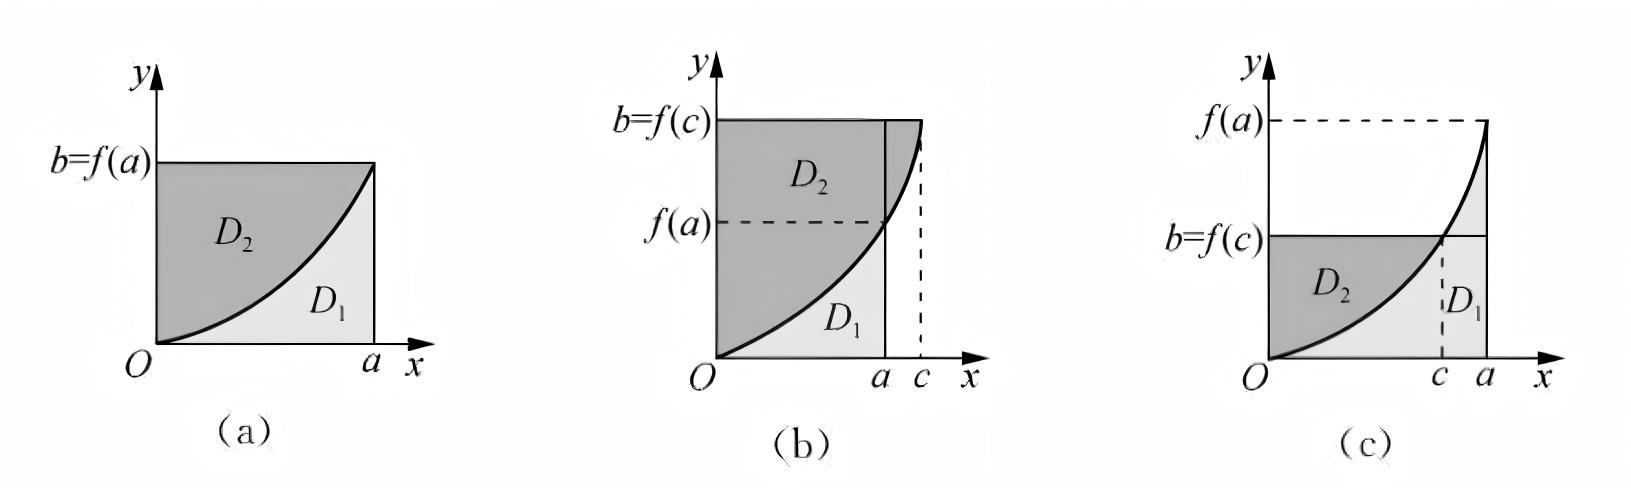
\includegraphics[width=0.7\linewidth]{figure/young}
	\end{center}
设 $f(a)=b$，取 $[0,a]$ 的划分：
	\[
	0 = x_0 < x_1 < \dots < x_n = a
	\]
	对应地令
	\[
	y_i = f(x_i)
	\]
	我们得到 $[0,b]$ 的划分
	\[
	0 = y_0 < y_1 < \dots < y_n = b
	\]
	那么
	\[
	\int_{0}^{a} f(x) \dd x = \sum_{i=1}^{n} y_{i-1} (x_i - x_{i-1}), \quad \int_{0}^{b} f^{-1}(x) \dd x = \sum_{i=1}^{n} x_i (y_i - y_{i-1})
	\]

	那么
	\begin{align*}
		\int_{0}^{a} f(x) \dd x + \int_{0}^{b} f^{-1}(x) \dd x
		&= \sum_{i=1}^{n} \left( x_i y_i - x_{i-1} y_{i-1} \right) \\
		&= x_n y_n - x_0 y_0 = ab
	\end{align*}
	
	若 $f(a) \neq b$，设 $f(T)=b$，令
	\[
	F(a) = \int_{0}^{a} f(x) \dd x + \int_{0}^{b} f^{-1}(x) \dd x - ab
	\]
	求导得
	\[
	F'(a) = f(a) - b
	\]
	
	\begin{itemize}
		\item 当 $a=T$ 时，$f(T)=b$，故 $F'(T)=0$
	 \item 当 $a>T$ 时，$f(a)>b$，故 $F'(a)>0$，$F(a)$ 单调递增
	\item 当 $a<T$ 时，$f(a)<b$，故 $F'(a)<0$，$F(a)$ 单调递减
	\end{itemize}
	
	故 $a=T$ 时 $F(a)$ 取得最小值，且 $F(T)=0$。因此 $\forall a$，有 $F(a) \geqslant 0$，也即
	\[
	\int_{0}^{a} f(x) \dd x + \int_{0}^{b} f^{-1}(x) \dd x \geqslant ab
	\]
\end{proof}
\begin{corollary}
	设 $p>1$，$q>1$ 且 $\dfrac{1}{p} + \dfrac{1}{q} = 1$，则 $\forall a,b \geqslant 0$，必有
	\[
	ab \leqslant \frac{a^p}{p} + \frac{b^q}{q}
	\]
\end{corollary}
\begin{proof}
	令 $y = x^{p-1}$，其反函数为 $x = y^{q-1}$。由Young不等式得
	\[
	\int_{0}^{a} x^{p-1} \dd x + \int_{0}^{b} x^{q-1} \dd x \geqslant ab
	\]
	计算积分即得
	\[
	ab \leqslant \frac{a^p}{p} + \frac{b^q}{q}
	\]
\end{proof}
\begin{corollary}
	（Hölder 不等式）设 $f,g \in C[a,b]$，$p,q>1$，且 $\dfrac{1}{p} + \dfrac{1}{q} = 1$，则
	\[
	\int_{a}^{b} |fg| \dd x \leqslant \left( \int_{a}^{b} |f|^p \dd x \right)^{\frac{1}{p}} \cdot \left( \int_{a}^{b} |g|^q \dd x \right)^{\frac{1}{q}}
	\]
	
若$p,q<1$，且 $\dfrac{1}{p} + \dfrac{1}{q} = 1$，则
\[
\int_{a}^{b} |fg| \dd x \geqslant \left( \int_{a}^{b} |f|^p \dd x \right)^{\frac{1}{p}} \cdot \left( \int_{a}^{b} |g|^q \dd x \right)^{\frac{1}{q}}
\]
	等号成立当且仅当$f^p(x)$与$g^q(x)$成比例时
\end{corollary}
\begin{proof}
	对任意 $\varphi(x),\psi(x) > 0$，$p,q>1$ 且 $\dfrac{1}{p} + \dfrac{1}{q} = 1$，有
	\[
	\varphi(x)\psi(x) \leqslant \frac{1}{p} \varphi(x)^p + \frac{1}{q} \psi(x)^q
	\]
	
	令
	\[
	\varphi(x) = \frac{|f(x)|}{\left( \displaystyle\int_{a}^{b} |f|^p \dd x \right)^{\frac{1}{p}}}, \quad
	\psi(x) = \frac{|g(x)|}{\left( \displaystyle\int_{a}^{b} |g|^q \dd x \right)^{\frac{1}{q}}}
	\]
	
	代入上述不等式，得
	\[
	\frac{|fg|}{\left( \displaystyle\int_{a}^{b} |f|^p \dd x \right)^{\frac{1}{p}} \left( \displaystyle\int_{a}^{b} |g|^q \dd x \right)^{\frac{1}{q}}}
	\leqslant \frac{|f|^p}{p \displaystyle\int_{a}^{b} |f|^p \dd x} + \frac{|g|^q}{q \displaystyle\int_{a}^{b} |g|^q \dd x}
	\]
	
	两边在 $[a,b]$ 上积分，整理后即得 Hölder 不等式。对称的证明类似
\end{proof}
\begin{corollary}
	(Minkowski不等式)$f,g\in\mathcal{R}[a,b]$且$f,g$的下界为正,则\[\sqrt[]{\int_{a}^{b}[f(x)+g(x)]^2\dd x}\leqslant \sqrt{\int_{a}^{b}f(x)\dd x}+\sqrt{\int_{a}^{b}g(x)\dd x}\]
\end{corollary}
\begin{proof}

	\[\begin{aligned}
			\int_{a}^{b}(f+g)^2\dd x&==2\int_{a}^{b}fg\dd x+\int_{a}^{b}f^2\dd x+\int_{a}^{b}g^2\dd x\\
			&\leqslant 2\sqrt{\int_{a}^{b}f^2\dd x\int_{a}^{b}g^2\dd x}+\int_{a}^{b}f^2\dd x+\int_{a}^{b}g^2\dd x\\
			&=(\sqrt[]{\int_{a}^{b}f^2\dd x}+\sqrt[]{\int_{a}^{b}g^2\dd x})^2
	\end{aligned}\]
\end{proof}
更进一步的，我们有
\begin{corollary}
	$f_i\in \mathcal{R}[a,b](i=1,\cdots,m)$，且下界为正，对$r>1$
	\[  \left[\int_{a}^{b}(f_1(x)+\cdots+f_m(x))^r\dd x\right]^{\frac{1}{r}}\leqslant (\int_{a}^{b}f_1^r(x)\dd x)^{\frac{1}{r}}+\cdots+(\int_{a}^{b}f_m^r(x)\dd x)^{\frac{1}{r}}  \]
	
	对$r<1$
	\[  \left[\int_{a}^{b}(f_1(x)+\cdots+f_m(x))^r\dd x\right]^{\frac{1}{r}}\geqslant (\int_{a}^{b}f_1^r(x)\dd x)^{\frac{1}{r}}+\cdots+(\int_{a}^{b}f_m^r(x)\dd x)^{\frac{1}{r}}  \]

\end{corollary}
%
% 第5节：中值定理
% !TEX root = ../../../main.tex
% 所属：第一部分：单变量分析学 / 第10章：一些定积分的问题
% 节：10.5 中值定理
% 正文按原文件顺序保存；由 ../chapter10.tex 调用。
\section{中值定理}

本节主要整理几道利用积分中值定理与 Rolle 中值定理的题目.

\begin{problem}
 设 $f(x)$ 在 $(0,1)$ 上可微，且满足
	\[
	f(1)-2\int_0^{\frac12}x f(x)\dd x=0.
	\]
	求证：在 $(0,1)$ 内至少有一点 $\xi$，使得
	\[
	f'(\xi)=-\frac{f(\xi)}{\xi}.
	\]
\end{problem}

\begin{proof}
	由积分中值定理，存在 $\eta\in\left(0,\dfrac12\right)$，使得
	\[
	\int_0^{\frac12}x f(x)\dd x=\frac12\eta f(\eta).
	\]
	因此
	\[
	f(1)=2\int_0^{\frac12}x f(x)\dd x=\eta f(\eta).
	\]
	令 $F(x)=x f(x)$，则
	\[
	F(1)=f(1)=\eta f(\eta)=F(\eta).
	\]
	于是对 $F(x)$ 在 $[\eta,1]$ 上应用 Rolle 中值定理，存在 $\xi\in(\eta,1)$，使得
	\[
	F'(\xi)=0.
	\]
	即
	\[
	f(\xi)+\xi f'(\xi)=0,
	\]
	所以
	\[
	f'(\xi)=-\frac{f(\xi)}{\xi}.
	\]
\end{proof}

\begin{problem}
设 $f(x)$ 在区间 $[0,1]$ 上连续，在 $(0,1)$ 上可导，满足
	\[
	f(1)=2\int_0^{\frac12}e^{1-x^2}f(x)\dd x.
	\]
	求证：存在一点 $\xi\in(0,1)$，使得
	\[
	f'(\xi)=2\xi f(\xi).
	\]
\end{problem}

\begin{proof}
	由题设两边同乘 $e^{-1}$ 得
	\[
	e^{-1}f(1)=2\int_0^{\frac12}e^{-x^2}f(x)\dd x.
	\]
	由积分中值定理，存在 $\eta\in\left(0,\dfrac12\right)$，使得
	\[
	2\int_0^{\frac12}e^{-x^2}f(x)\dd x=e^{-\eta^2}f(\eta).
	\]
	于是
	\[
	e^{-1}f(1)=e^{-\eta^2}f(\eta).
	\]
	令
	\[
	F(x)=e^{-x^2}f(x),
	\]
	则 $F(1)=F(\eta)$，由 Rolle 中值定理，存在 $\xi\in(\eta,1)$，使得
	\[
	F'(\xi)=0.
	\]
	又
	\[
	F'(x)=e^{-x^2}\left(f'(x)-2x f(x)\right),
	\]
	故
	\[
	f'(\xi)-2\xi f(\xi)=0,
	\]
	即
	\[
	f'(\xi)=2\xi f(\xi).
	\]
\end{proof}

\begin{problem}
设 $f(x)$ 在 $[0,1]$ 上连续，在 $(0,1)$ 内三次可微，并且满足条件：
	\[
	\int_0^{\frac14}f(t)\dd t=\frac14 f(0),
	\qquad
	\int_{\frac14}^{1}f(t)\dd t=\frac34 f(1).
	\]
	试证：若 $f(0)=f(1)$，则存在 $\xi\in(0,1)$，使得
	\[
	f'''(\xi)=0.
	\]
\end{problem}

\begin{proof}
	由积分中值定理，存在 $\xi_1\in\left(0,\dfrac14\right)$，使得
	\[
	\int_0^{\frac14}f(t)\dd t=\frac14 f(\xi_1).
	\]
	结合题设得
	\[
	f(\xi_1)=f(0).
	\]
	同理，存在 $\xi_2\in\left(\dfrac14,1\right)$，使得
	\[
	\int_{\frac14}^{1}f(t)\dd t=\frac34 f(\xi_2),
	\]
	从而
	\[
	f(\xi_2)=f(1).
	\]
	又 $f(0)=f(1)$，所以
	\[
	f(0)=f(\xi_1)=f(\xi_2)=f(1).
	\]
	于是分别在 $[0,\xi_1]$，$[\xi_1,\xi_2]$，$[\xi_2,1]$ 上应用 Rolle 中值定理，存在
	\[
	\eta_1\in(0,\xi_1),\qquad
	\eta_2\in(\xi_1,\xi_2),\qquad
	\eta_3\in(\xi_2,1),
	\]
	使得
	\[
	f'(\eta_1)=f'(\eta_2)=f'(\eta_3)=0.
	\]
	再对 $f'(x)$ 分别在 $[\eta_1,\eta_2]$ 与 $[\eta_2,\eta_3]$ 上应用 Rolle 中值定理，存在
	\[
	\delta_1\in(\eta_1,\eta_2),
	\qquad
	\delta_2\in(\eta_2,\eta_3),
	\]
	使得
	\[
	f''(\delta_1)=f''(\delta_2)=0.
	\]
	最后对 $f''(x)$ 在 $[\delta_1,\delta_2]$ 上应用 Rolle 中值定理，存在 $\xi\in(\delta_1,\delta_2)$，使得
	\[
	f'''(\xi)=0.
	\]
\end{proof}

\begin{problem}
	设函数 $f(x)$ 在 $[0,\pi]$ 上连续，且
	\[
	\int_0^\pi f(x)\dd x=0,
	\qquad
	\int_0^\pi f(x)\cos x\dd x=0.
	\]
	证明：在 $(0,\pi)$ 内至少存在两个不同的点 $\xi_1,\xi_2$，使得
	\[
	f(\xi_1)=f(\xi_2)=0.
	\]
\end{problem}

\begin{proof}
	令
	\[
	g(x)=\int_0^x f(t)\dd t,
	\qquad
	h(x)=\int_0^x g(t)\sin t\dd t.
	\]
	由题设知
	\[
	g(0)=g(\pi)=0,
	\qquad
	h(0)=0.
	\]
	又由分部积分，
	\[
	\begin{aligned}
		h(\pi)
		&=\int_0^\pi g(x)\sin x\dd x \\
		&=\left[-g(x)\cos x\right]_0^\pi+
		\int_0^\pi f(x)\cos x\dd x=0.
	\end{aligned}
	\]
	于是 $h(0)=h(\pi)=0$，由 Rolle 中值定理，存在 $\eta\in(0,\pi)$，使得
	\[
	h'(\eta)=g(\eta)\sin\eta=0.
	\]
	由于 $\eta\in(0,\pi)$，故 $\sin\eta>0$，从而
	\[
	g(\eta)=0.
	\]
	因此
	\[
	g(0)=g(\eta)=g(\pi)=0.
	\]
	分别对 $g(x)$ 在 $[0,\eta]$ 与 $[\eta,\pi]$ 上应用 Rolle 中值定理，存在
	\[
	\xi_1\in(0,\eta),
	\qquad
	\xi_2\in(\eta,\pi),
	\]
	使得
	\[
	g'(\xi_1)=g'(\xi_2)=0.
	\]
	又 $g'(x)=f(x)$，所以
	\[
	f(\xi_1)=f(\xi_2)=0.
	\]
	显然 $\xi_1\neq\xi_2$.
\end{proof}

%
% 第6节：定积分的数值积分-算法与编程
% !TEX root = ../../../main.tex
% 所属：第一部分：单变量分析学 / 第10章：一些定积分的问题
% 节：10.6 定积分的数值积分-算法与编程
% 正文按原文件顺序保存；由 ../chapter10.tex 调用。
\section{定积分的数值积分-算法与编程}
本节讨论若干常用的数值积分公式。基本思想是：在积分区间上先用多项式近似被积函数，再对这个多项式进行积分，从而得到原积分的近似值。

\subsection*{Newton--Cotes 求积公式}

将积分区间 $[a,b]$ 以步长
\[
h=\frac{b-a}{n}
\]
分成 $n$ 等份。

取分点
\[
x_i=a+ih,\qquad i=0,1,2,\dots,n.
\]

以这些分点为节点，作 $f(x)$ 的 Lagrange 插值多项式
\[
f(x)\approx p_n(x)
=\sum_{i=0}^{n}\left(\prod_{\substack{j=0\\j\ne i}}^{n}
\frac{x-x_j}{x_i-x_j}\right)f(x_i).
\]

对等式两边在 $[a,b]$ 上积分，得到
\[
\int_a^b f(x)\dd x
\approx \int_a^b p_n(x)\dd x
=(b-a)\sum_{i=0}^{n} C_i^{(n)}f(x_i).
\]

其中
\[
\begin{aligned}
	C_i^{(n)}
	&=\frac1{b-a}\int_a^b
	\prod_{\substack{j=0\\j\ne i}}^n\frac{x-x_j}{x_i-x_j}\dd x \\[4pt]
	&=\frac{h}{b-a}\int_0^n
	\prod_{\substack{j=0\\j\ne i}}^n\frac{t-j}{i-j}\dd t
	\qquad (x=a+th) \\[4pt]
	&=\frac1n\cdot \frac{(-1)^{n-i}}{i!(n-i)!}
	\int_0^n\prod_{\substack{j=0\\j\ne i}}^n(t-j)\dd t.
\end{aligned}
\]

这就是 $n$ 步 Newton--Cotes 求积公式。计算时需要 $n+1$ 个节点，相应的 $C_i^{(n)}$ 称为 Cotes 系数。它与积分区间和被积函数无关，只依赖于所取的节点个数，因此可以预先由多项式积分算出。

\begin{example}
	\textbf{梯形公式.}
	当 $n=1$ 时，由 Cotes 系数的性质，得到
	\[
	C_0^{(1)}=C_1^{(1)}=\frac12.
	\]因此
	\[
	\int_a^b f(x)\dd x
	\approx \frac{b-a}{2}\bigl[f(a)+f(b)\bigr].
	\]
	这称为梯形公式。
\end{example}
使用Python我们可以使用以下的代码进行计算
\begin{verbatim}
	import sympy
	from sympy import symbols, sympify, lambdify
	def trapezoidal_rule(f, a: float, b: float) -> float:
	return (b - a) / 2.0 * (f(a) + f(b))
	if __name__ == "__main__":
	x = symbols('x')
	expr_str = input("请输入函数表达式（例如：x**2 + sin(x)）：")
	expr = sympify(expr_str)
	a = float(input("请输入积分下限 a = "))
	b = float(input("请输入积分上限 b = "))
	f = lambdify(x, expr, modules="math")
	result = trapezoidal_rule(f, a, b)
	print(f"\n梯形公式近似值: {result:.10f}")
\end{verbatim}
\begin{example}
	\textbf{Simpson 公式.}
	当 $n=2$ 时，
	\[
	C_0^{(2)}=\frac14\int_0^2(t-1)(t-2)\dd t
	=\frac16=C_2^{(2)},
	\]
	因此得到 Simpson 公式
	\[
	\int_a^b f(x)\dd x
	\approx \frac{b-a}{6}
	\left[f(a)+4f\left(\frac{a+b}{2}\right)+f(b)\right].
	\]
\end{example}
使用Python我们可以使用以下的代码进行计算
\begin{verbatim}
	import sympy
	from sympy import symbols, sympify, lambdify
	def simpson_rule(f, a: float, b: float) -> float:
	mid = (a + b) / 2.0
	return (b - a) / 6.0 * (f(a) + 4.0 * f(mid) + f(b))
	if __name__ == "__main__":
	x = symbols('x')
	expr_str = input("请输入函数表达式（例如：x**2 + sin(x)）：")
	expr = sympify(expr_str)
	a = float(input("请输入积分下限 a = "))
	b = float(input("请输入积分上限 b = "))
	f = lambdify(x, expr, modules="math")
	result = simpson_rule(f, a, b)
	print(f"\nSimpson 公式近似值: {result:.10f}")
\end{verbatim}

\begin{example}
	\textbf{Cotes 公式.}
	当 $n=4$ 时，
	\[
	\begin{aligned}
		C_0^{(4)}
		&=\frac1{96}\int_0^4(t-1)(t-2)(t-3)(t-4)\dd t
		=\frac7{90}=C_4^{(4)},\\[4pt]
		C_1^{(4)}
		&=-\frac1{24}\int_0^4t(t-2)(t-3)(t-4)\dd t
		=\frac{32}{90}=C_3^{(4)},\\[4pt]
		C_2^{(4)}
		&=1-2\left(C_0^{(4)}+C_1^{(4)}\right)=\frac{12}{90}.
	\end{aligned}
	\]
	于是得到 Cotes 公式
	\[
	\int_a^b f(x)\dd x
	\approx \frac{b-a}{90}
	\left\{7\bigl[f(x_0)+f(x_4)\bigr]
	+32\bigl[f(x_1)+f(x_3)\bigr]+12f(x_2)\right\},
	\]
	其中
	\[
	x_i=\frac{(4-i)a+ib}{4},\qquad i=0,1,2,3,4.
	\]
	
\end{example}
使用Python我们可以使用以下的代码进行计算
\begin{verbatim}
	import sympy
	from sympy import symbols, sympify, lambdify
	def cotes_rule(f, a: float, b: float) -> float:
	n = 4
	x = [((n - i) * a + i * b) / n for i in range(n + 1)]
	C = [7/90, 32/90, 12/90, 32/90, 7/90]
	s = sum(C[i] * f(x[i]) for i in range(n + 1))
	return (b - a) * s
	if __name__ == "__main__":
	x = symbols('x')
	expr_str = input("请输入函数表达式（例如：x**2 + sin(x)）：")
	expr = sympify(expr_str)
	a = float(input("请输入积分下限 a = "))
	b = float(input("请输入积分上限 b = "))
	f = lambdify(x, expr, modules="math")
	result = cotes_rule(f, a, b)
	print(f"\nCotes 公式近似值: {result:.10f}")
\end{verbatim}


\subsection*{复化公式}

单一区间上的求积公式通常只利用少数节点。为了提高近似效果，可以先把 $[a,b]$ 划分为若干小区间，再在每个小区间上使用相同的求积公式，最后把各小区间的结果相加。这类公式称为复化求积公式。


	\textbf{复化梯形公式.}
	将 $[a,b]$ 以步长
	\[
	h=\frac{b-a}{m}
	\]
	作 $m$ 等分。

记
\[
x_i=a+ih,\qquad i=0,1,2,\dots,m.
\]

在每一个小区间 $[x_{i-1},x_i]$ 上使用梯形公式，得到
\[
\begin{aligned}
	\int_a^b f(x)\dd x
	&=\sum_{i=1}^{m}\int_{x_{i-1}}^{x_i}f(x)\dd x \\[2pt]
	&\approx \frac{h}{2}\sum_{i=1}^{m}
	\bigl[f(x_{i-1})+f(x_i)\bigr].
\end{aligned}
\]

记
\[
T_m^{(1)}
=\frac{h}{2}\left[f(a)+f(b)+2\sum_{i=1}^{m-1}f(x_i)\right],
\]
则称 $T_m^{(1)}$ 为将区间 $m$ 等分的复化梯形公式。

使用Python我们可以使用以下的代码进行计算
\begin{verbatim}
	import sympy
	from sympy import symbols, sympify, lambdify
	def composite_trapezoidal_rule(f, a: float, b: float, m: int) -> float:
	h = (b - a) / m
	s = f(a) + f(b)
	for i in range(1, m):
	s += 2.0 * f(a + i * h)
	return (h / 2.0) * s
	if __name__ == "__main__":
	x = symbols('x')
	expr_str = input("请输入函数表达式（例如：x**2 + sin(x)）：")
	expr = sympify(expr_str)
	a = float(input("请输入积分下限 a = "))
	b = float(input("请输入积分上限 b = "))
	m = int(input("请输入等分数 m = "))
	f = lambdify(x, expr, modules="math")
	result = composite_trapezoidal_rule(f, a, b, m)
	print(f"\n复化梯形公式近似值: {result:.10f}")
	
\end{verbatim}
	\textbf{复化 Simpson 公式.}
	记
	\[
	x_{i-\frac12}=\frac{x_{i-1}+x_i}{2}
	\]
	为区间 $[x_{i-1},x_i]$ 的中点。


在每个小区间上使用 Simpson 公式，可以得到复化 Simpson 公式
\[
\begin{aligned}
	T_m^{(2)}=S_m
	&=\frac{h}{6}\sum_{i=1}^{m}
	\left[f(x_{i-1})+4f\left(x_{i-\frac12}\right)+f(x_i)\right] \\[4pt]
	&=\frac{h}{6}\left[f(a)+f(b)
	+2\sum_{i=1}^{m-1}f(x_i)
	+4\sum_{i=1}^{m}f\left(x_{i-\frac12}\right)\right].
\end{aligned}
\]
使用Python我们可以使用以下的代码进行计算
\begin{verbatim}
	import sympy
	from sympy import symbols, sympify, lambdify
	def composite_simpson_rule(f, a: float, b: float, m: int) -> float:
	h = (b - a) / m
	s = f(a) + f(b)
	for i in range(1, m):
	s += 2.0 * f(a + i * h)
	for i in range(1, m + 1):
	s += 4.0 * f(a + (i - 0.5) * h)
	return (h / 6.0) * s
	if __name__ == "__main__":
	x = symbols('x')
	expr_str = input("请输入函数表达式（例如：x**2 + sin(x)）：")
	expr = sympify(expr_str)
	a = float(input("请输入积分下限 a = "))
	b = float(input("请输入积分上限 b = "))
	m = int(input("请输入等分数 m = "))
	f = lambdify(x, expr, modules="math")
	result = composite_simpson_rule(f, a, b, m)
	print(f"\n复化 Simpson 公式近似值: {result:.10f}")
\end{verbatim}
	\textbf{复化 Cotes 公式.}
	在每个小区间 $[x_{i-1},x_i]$ 上使用四等分的 Cotes 公式。令
	\[
	y_{i,r}=x_{i-1}+\frac{r}{4}h,
	\qquad r=0,1,2,3,4,
	\]


则复化 Cotes 公式可以写为
\[
\begin{aligned}
	C_m
	=\frac{h}{90}\sum_{i=1}^{m}
	\bigl\{&7\bigl[f(y_{i,0})+f(y_{i,4})\bigr]
	+32\bigl[f(y_{i,1})+f(y_{i,3})\bigr] \\
	&+12f(y_{i,2})\bigr\}.
\end{aligned}
\]
使用Python我们可以使用以下的代码进行计算
\begin{verbatim}
	import sympy
	from sympy import symbols, sympify, lambdify
	def composite_cotes_rule(f, a: float, b: float, m: int) -> float:
	h = (b - a) / m
	s = 0.0
	for i in range(1, m + 1):
	x0 = a + (i - 1) * h        # y_{i,0}
	x1 = x0 + h / 4.0           # y_{i,1}
	x2 = x0 + h / 2.0           # y_{i,2}
	x3 = x0 + 3.0 * h / 4.0     # y_{i,3}
	x4 = x0 + h                 # y_{i,4}
	s += 7.0 * (f(x0) + f(x4)) + 32.0 * (f(x1) + f(x3)) + 12.0 * f(x2)
	return (h / 90.0) * s
	if __name__ == "__main__":
	x = symbols('x')
	expr_str = input("请输入函数表达式（例如：x**2 + sin(x)）：")
	expr = sympify(expr_str)
	a = float(input("请输入积分下限 a = "))
	b = float(input("请输入积分上限 b = "))
	m = int(input("请输入等分数 m = "))
	f = lambdify(x, expr, modules="math")
	result = composite_cotes_rule(f, a, b, m)
	print(f"\n复化 Cotes 公式近似值: {result:.10f}")
\end{verbatim}
\subsection*{Romberg 方法}

把上面的外推思想推广到一般的 $T_m^{(k)}$。记
\[
T_m^{(k+1)}
=\frac{4^kT_{2m}^{(k)}-T_m^{(k)}}{4^k-1}.
\]

这就得到数值积分的 Romberg 方法。它的计算过程可以按如下图式进行：先取适当的初始值 $m$，再依次逐个计算。向下的箭头表示把区间再细化一半，向右的箭头表示外推。

\providecommand{\rombergstep}[1]{\tikz[baseline=(char.base)]{\node[draw,circle,inner sep=0.5pt,font=\scriptsize] (char) {#1};}}

\begin{figure}[H]
	\centering
	\begin{tikzpicture}[>=Stealth, node distance=1.15cm and 2.05cm]
		\node (a1) at (0,0) {$T_m^{(1)}$};
		\node (a2) at (0,-1.25) {$T_{2m}^{(1)}$};
		\node (a3) at (0,-2.50) {$T_{4m}^{(1)}$};
		\node (a4) at (0,-3.75) {$T_{8m}^{(1)}$};
		
		\node (b1) at (2.35,-0.625) {$T_m^{(2)}$};
		\node (b2) at (2.35,-1.875) {$T_{2m}^{(2)}$};
		\node (b3) at (2.35,-3.125) {$T_{4m}^{(2)}$};
		
		\node (c1) at (4.70,-1.25) {$T_m^{(3)}$};
		\node (c2) at (4.70,-2.50) {$T_{2m}^{(3)}$};
		
		\node (d1) at (7.05,-1.875) {$T_m^{(4)}$};
		
		\draw[->] (a1)--(a2);
		\draw[->] (a2)--(a3);
		\draw[->] (a3)--(a4);
		
		\draw[->] (a1)--(b1);
		\draw[->] (a2)--(b1);
		\draw[->] (a2)--(b2);
		\draw[->] (a3)--(b2);
		\draw[->] (a3)--(b3);
		\draw[->] (a4)--(b3);
		\draw[->] (b1)--(b2);
		\draw[->] (b2)--(b3);
		
		\draw[->] (b1)--(c1);
		\draw[->] (b2)--(c1);
		\draw[->] (b2)--(c2);
		\draw[->] (b3)--(c2);
		\draw[->] (c1)--(c2);
		
		\draw[->] (c1)--(d1);
		\draw[->] (c2)--(d1);
		
		\node at (-0.45,0.25) {\rombergstep{1}};
		\node at (-0.45,-1.00) {\rombergstep{2}};
		\node at (1.70,-0.40) {\rombergstep{3}};
		\node at (-0.45,-2.25) {\rombergstep{4}};
		\node at (1.70,-1.65) {\rombergstep{5}};
		\node at (4.05,-1.02) {\rombergstep{6}};
		\node at (-0.45,-3.50) {\rombergstep{7}};
		\node at (1.70,-2.90) {\rombergstep{8}};
		\node at (4.05,-2.27) {\rombergstep{9}};
		\node at (6.40,-1.65) {\rombergstep{10}};
		
		\node at (0,-4.45) {$\vdots$};
	\end{tikzpicture}
	\caption{Romberg 方法的计算顺序示意图}
\end{figure}

在实际计算中，一般从 $m=1$、$k=1$ 开始逐步计算 $T_m^{(k)}$。若对某个 $k$ 有 $|T_m^{(k)}-T_{m/2}^{(k)}|$ 小于预先设定的精度要求，就可把相应结果作为积分的近似值；否则继续把小区间长度缩小二分之一，计算出新的数值并继续比较。这种根据预置精度要求、在计算过程中自动把区间划分到合适程度的算法，称为自适应算法。
%
% 第7节：定积分的几何应用
% !TEX root = ../../../main.tex
% 所属：第一部分：单变量分析学 / 第10章：一些定积分的问题
% 节：10.7 定积分的几何应用
% 正文按原文件顺序保存；由 ../chapter10.tex 调用。
\section{定积分的几何应用}
本节整理定积分在几何问题中的若干基本应用。
\subsection*{平面图形的面积}

\begin{proposition}[直角坐标下的曲边梯形面积]
	设 $f$ 在 $[a,b]$ 上连续。
	\begin{enumerate}
		\item 若 $f(x)\geq 0$，则由 $y=f(x)$、$x=a$、$x=b$ 与 $x$ 轴围成的曲边梯形面积为
		\[
		S=\int_a^b f(x)\dd x .
		\]
		\item 若 $f(x)\leq 0$，则对应面积为
		\[
		S=-\int_a^b f(x)\dd x=\int_a^b \abs{f(x)}\dd x .
		\]
		\item 一般地，若 $f$ 在区间内可能变号，则面积为
		\[
		S=\int_a^b \abs{f(x)}\dd x .
		\]
	\end{enumerate}
\end{proposition}

\begin{proof}
	当 $f(x)\geq 0$ 时，面积由 Riemann 和
	\[
	\sum_{i=1}^n f(\xi_i)\Delta x_i
	\]
	的极限给出，因此为 $\displaystyle\int_a^b f(x)\dd x$。若 $f(x)\leq 0$，图形在 $x$ 轴下方，几何面积应取正值，故为 $-\displaystyle\int_a^b f(x)\dd x$。若 $f$ 有变号点，则把 $[a,b]$ 按变号点分成有限个小区间，在每段分别应用前两种情形，合并后得到
	\[
	S=\int_a^b \abs{f(x)}\dd x .
	\]
\end{proof}

\begin{figure}[H]
	\begin{center}
		\begin{tikzpicture}[scale=1.05,>=Stealth]
			\draw[->] (-0.3,0) -- (3.6,0) node[right] {$x$};
			\draw[->] (0,-0.25) -- (0,2.25) node[above] {$y$};
			\fill[blue!12] (0,0) -- plot[domain=0:3,samples=80] ({\x},{0.75+0.75*\x-0.16*\x*\x}) -- (3,0) -- cycle;
			\draw[thick,blue!70!black,domain=0:3,samples=80] plot ({\x},{0.75+0.75*\x-0.16*\x*\x});
			\draw[dashed] (0,0) -- (0,{0.75});
			\draw[dashed] (3,0) -- (3,{0.75+0.75*3-0.16*9});
			\fill[blue!30] (1.05,0) rectangle (1.35,{0.75+0.75*1.2-0.16*1.2*1.2});
			\fill[blue!30] (1.75,0) rectangle (2.05,{0.75+0.75*1.9-0.16*1.9*1.9});
			\draw[blue!70!black] (1.05,0) rectangle (1.35,{0.75+0.75*1.2-0.16*1.2*1.2});
			\draw[blue!70!black] (1.75,0) rectangle (2.05,{0.75+0.75*1.9-0.16*1.9*1.9});
			\node[below] at (0,0) {$a$};
			\node[below] at (3,0) {$b$};
			\node[above right] at (2.05,1.55) {$y=f(x)\geq 0$};
			\node at (1.62,0.55) {$S=\displaystyle\int_a^b f(x)\dd x$};
			\node[below] at (1.20,-0.05) {$\Delta x_i$};
			\node[above] at (1.20,1.30) {$f(\xi_i)$};
		\end{tikzpicture}
	\end{center}
	\caption{曲边梯形面积：用小矩形面积之和逼近曲线下方区域。}
\end{figure}


\begin{proposition}[两条曲线之间的面积]
	设 $f,g$ 在 $[a,b]$ 上连续，且 $f(x)\geq g(x)$。则由 $y=f(x)$、$y=g(x)$、$x=a$ 与 $x=b$ 围成的平面图形面积为
	\[
	S=\int_a^b \bigl[f(x)-g(x)\bigr]\dd x .
	\]
	更一般地，若两曲线在区间内有交点，则应按交点分段；等价地可以写成
	\[
	S=\int_a^b \abs{f(x)-g(x)}\dd x .
	\]
\end{proposition}

\begin{proof}
	在每个小区间 $[x_{i-1},x_i]$ 上，面积近似为高为 $f(\xi_i)-g(\xi_i)$、宽为 $\Delta x_i$ 的小矩形面积，故
	\[
	S\approx \sum_{i=1}^n \bigl[f(\xi_i)-g(\xi_i)\bigr]\Delta x_i .
	\]
	令分割的最大长度趋于 $0$，由定积分定义得
	\[
	S=\int_a^b \bigl[f(x)-g(x)\bigr]\dd x .
	\]
	若上下关系发生改变，则在交点处分段，合并后得到绝对值形式。
\end{proof}

\begin{figure}[H]
	\begin{center}
		\begin{tikzpicture}[scale=1.05,>=Stealth]
			\draw[->] (-0.3,0) -- (3.6,0) node[right] {$x$};
			\draw[->] (0,-0.25) -- (0,2.35) node[above] {$y$};
			\fill[orange!18] plot[domain=0:3,samples=80] ({\x},{1.85-0.18*(\x-1.5)*(\x-1.5)}) --
			plot[domain=3:0,samples=80] ({\x},{0.45+0.20*\x}) -- cycle;
			\draw[thick,red!70!black,domain=0:3,samples=80] plot ({\x},{1.85-0.18*(\x-1.5)*(\x-1.5)});
			\draw[thick,green!45!black,domain=0:3,samples=80] plot ({\x},{0.45+0.20*\x});
			\draw[dashed] (0,0) -- (0,{1.85-0.18*2.25});
			\draw[dashed] (3,0) -- (3,{1.85-0.18*2.25});
			\draw[<->] (1.5,{0.45+0.20*1.5}) -- (1.5,{1.85});
			\node[right] at (1.5,1.15) {$f(x)-g(x)$};
			\node[above] at (2.25,1.72) {$y=f(x)$};
			\node[below right] at (2.0,0.85) {$y=g(x)$};
			\node[below] at (0,0) {$a$};
			\node[below] at (3,0) {$b$};
			\node at (1.45,0.35) {$S=\displaystyle\int_a^b [f(x)-g(x)]\dd x$};
		\end{tikzpicture}
	\end{center}
	\caption{两条曲线之间的面积：小矩形的高为上曲线与下曲线的函数值之差。}
\end{figure}


\begin{proposition}[参数方程下的面积]
	设曲线由参数方程
	\[
	x=x(t),\qquad y=y(t),\qquad t\in[\alpha,\beta]
	\]
	给出，其中 $x,y$ 连续可微，且 $x(t)$ 在 $[\alpha,\beta]$ 上单调。若曲线与 $x$ 轴围成的区域位于 $x$ 轴同侧，则面积可写为
	\[
	S=\int_{\alpha}^{\beta}\abs{y(t)x'(t)}\dd t .
	\]
	若已经知道 $x'(t)\geq 0$，则
	\[
	S=\int_{\alpha}^{\beta} y(t)x'(t)\dd t;
	\]
	若 $x'(t)\leq 0$，则
	\[
	S=-\int_{\alpha}^{\beta} y(t)x'(t)\dd t .
	\]
\end{proposition}
\begin{proposition}[极坐标下的面积]
	设平面曲线由极坐标方程
	\[
	r=r(\theta),\qquad \theta\in[\alpha,\beta]
	\]
	给出。若曲线在该角区间内围成的区域可由射线角度单调扫过，则面积为
	\[
	S=\frac12\int_{\alpha}^{\beta}r^2(\theta)\dd\theta .
	\]
\end{proposition}
\begin{figure}[H]
	\begin{center}
		\begin{tikzpicture}[scale=1.0,>=Stealth]
			\begin{scope}
				\draw[->] (-0.2,0) -- (3.3,0) node[right] {$x$};
				\draw[->] (0,-0.2) -- (0,2.4) node[above] {$y$};
				\fill[blue!12] (0.35,0) -- plot[domain=0:3,samples=80] ({0.35+\x},{0.55+0.55*sin(55*\x)+0.25*\x}) -- (3.35,0) -- cycle;
				\draw[thick,blue!70!black,domain=0:3,samples=80] plot ({0.35+\x},{0.55+0.55*sin(55*\x)+0.25*\x});
				\node[below] at (0.35,0) {$x(\alpha)$};
				\node[below] at (3.35,0) {$x(\beta)$};
				\node at (1.8,0.45) {$S=\displaystyle\int_\alpha^\beta |y(t)x'(t)|\dd t$};
				\node[above] at (1.8,2.15) {参数方程面积};
			\end{scope}
			\begin{scope}[xshift=5.2cm]
				\draw[->] (-0.2,0) -- (3.0,0) node[right] {$x$};
				\draw[->] (0,-0.2) -- (0,2.6) node[above] {$y$};
				\fill[green!18] (0,0) -- plot[domain=25:125,variable=\t,samples=120]
				({(1.65+0.28*sin(2*\t))*cos(\t)},{(1.65+0.28*sin(2*\t))*sin(\t)}) -- cycle;
				\draw[thick,green!45!black,domain=25:125,variable=\t,samples=120]
				plot ({(1.65+0.28*sin(2*\t))*cos(\t)},{(1.65+0.28*sin(2*\t))*sin(\t)});
				\draw[thick] (0,0) -- ({(1.65+0.28*sin(50))*cos(25)},{(1.65+0.28*sin(50))*sin(25)});
				\draw[thick] (0,0) -- ({(1.65+0.28*sin(250))*cos(125)},{(1.65+0.28*sin(250))*sin(125)});
				\draw[->] (0.75,0) arc (0:25:0.75);
				\draw[->] (0.95,0) arc (0:125:0.95);
				\node at (0.95,0.25) {$\alpha$};
				\node at (-0.45,1.08) {$\beta$};
				\node at (0.8,1.05) {$r(\theta)$};
				\node[above] at (0.95,2.35) {极坐标面积};
				\node at (1.1,-0.35) {$S=\displaystyle\frac12\int_\alpha^\beta r^2(\theta)\dd\theta$};
			\end{scope}
		\end{tikzpicture}
	\end{center}
	\caption{参数方程面积与极坐标面积的图形来源。左图来自变量代换 $\dd x=x'(t)\dd t$；右图来自小扇形面积 $\frac12 r^2\Delta\theta$。}
\end{figure}
\newpage

\subsection*{曲线弧长}

\begin{proposition}[显式方程的弧长]
	设 $f$ 在 $[a,b]$ 上连续可微。曲线 $y=f(x)$ 在 $[a,b]$ 上的弧长为
	\[
	L=\int_a^b \sqrt{1+\bigl(f'(x)\bigr)^2}\dd x .
	\]
	对应的弧长微分为
	\[
	\dd l=\sqrt{1+\bigl(f'(x)\bigr)^2}\dd x .
	\]
\end{proposition}

\begin{proof}
	取分割
	\[
	a=x_0<x_1<\cdots<x_n=b .
	\]
	在小区间 $[x_{i-1},x_i]$ 上，用两端点连线长度近似曲线弧长，则
	\[
	\Delta l_i\approx
	\sqrt{(x_i-x_{i-1})^2+\bigl(f(x_i)-f(x_{i-1})\bigr)^2} .
	\]
	由 Lagrange 中值定理，存在 $\xi_i\in(x_{i-1},x_i)$，使得
	\[
	f(x_i)-f(x_{i-1})=f'(\xi_i)(x_i-x_{i-1}).
	\]
	因此
	\[
	\Delta l_i\approx \sqrt{1+\bigl(f'(\xi_i)\bigr)^2}\Delta x_i .
	\]
	求和并令分割最大长度趋于 $0$，得到
	\[
	L=\int_a^b \sqrt{1+\bigl(f'(x)\bigr)^2}\dd x .
	\]
\end{proof}

\begin{figure}[H]
	\begin{center}
		\begin{tikzpicture}[scale=1.05,>=Stealth]
			\draw[->] (-0.2,0) -- (4.4,0) node[right] {$x$};
			\draw[->] (0,-0.2) -- (0,2.6) node[above] {$y$};
			\draw[thick,blue!70!black,domain=0:4,samples=120] plot ({\x},{0.55+0.33*\x+0.28*sin(90*\x)});
			\draw[red!70!black,thick] (0,{0.55}) -- (1,{0.55+0.33+0.28*sin(90)});
			\draw[red!70!black,thick] (1,{0.55+0.33+0.28*sin(90)}) -- (2,{0.55+0.66+0.28*sin(180)});
			\draw[red!70!black,thick] (2,{0.55+0.66+0.28*sin(180)}) -- (3,{0.55+0.99+0.28*sin(270)});
			\draw[red!70!black,thick] (3,{0.55+0.99+0.28*sin(270)}) -- (4,{0.55+1.32+0.28*sin(360)});
			\node[above] at (2.65,0.8) {$y=f(x)$};
			\node[below] at (2.3,0.65) {折线长度 $\longrightarrow$ 曲线弧长};
			\node at (2.25,2.35) {$L=\displaystyle\int_a^b\sqrt{1+[f'(x)]^2}\dd x$};
		\end{tikzpicture}
	\end{center}
	\caption{显式方程弧长：先用相邻分点连成的折线近似曲线，再令分割加细。}
\end{figure}


\begin{proposition}[参数方程的弧长]
	设曲线由
	\[
	x=x(t),\qquad y=y(t),\qquad t\in[\alpha,\beta]
	\]
	给出，其中 $x,y$ 连续可微。若曲线无重复地由参数扫过，则其弧长为
	\[
	L=\int_{\alpha}^{\beta}
	\sqrt{\bigl(x'(t)\bigr)^2+\bigl(y'(t)\bigr)^2}\dd t .
	\]
	对应的弧长微分为
	\[
	\dd l=\sqrt{\bigl(x'(t)\bigr)^2+\bigl(y'(t)\bigr)^2}\dd t .
	\]
\end{proposition}
\begin{proposition}[极坐标方程的弧长]
	设曲线由
	\[
	r=r(\theta),\qquad \theta\in[\alpha,\beta]
	\]
	给出，其中 $r$ 连续可微。则弧长为
	\[
	L=\int_{\alpha}^{\beta}
	\sqrt{r^2(\theta)+\bigl(r'(\theta)\bigr)^2}\dd\theta .
	\]
	对应的弧长微分为
	\[
	\dd l=\sqrt{r^2(\theta)+\bigl(r'(\theta)\bigr)^2}\dd\theta .
	\]
\end{proposition}
\begin{example}[椭圆周长]
	设椭圆
	\[
	\frac{x^2}{a^2}+\frac{y^2}{b^2}=1,
	\qquad a>b>0,
	\]
	取参数方程
	\[
	x=a\cos t,
	\qquad
	y=b\sin t,
	\qquad 0\leq t\leq 2\pi .
	\]
	则
	\[
	\begin{aligned}
		L
		&=\int_0^{2\pi}\sqrt{a^2\sin^2t+b^2\cos^2t}\dd t \\
		&=a\int_0^{2\pi}\sqrt{1-k^2\cos^2t}\dd t,
		\qquad k=\frac{\sqrt{a^2-b^2}}{a} \\
		&=4a\int_0^{\frac{\pi}{2}}\sqrt{1-k^2\sin^2u}\dd u .
	\end{aligned}
	\]
	若记
	\[
	E(k,\varphi)=\int_0^{\varphi}\sqrt{1-k^2\sin^2u}\dd u,
	\]
	则 $E(k,\varphi)$ 称为第二类不完全椭圆积分；若进一步记
	\[
	E(k)=E\left(k,\frac{\pi}{2}\right),
	\]
	则椭圆周长可写为
	\[
	L=4aE(k).
	\]
\end{example}

\subsection*{旋转体体积}

\begin{proposition}[已知截面积的体积]
	设立体在垂直于 $x$ 轴的截面面积为 $A(x)$，其中 $x\in[a,b]$。若 $A$ 在 $[a,b]$ 上连续，则立体体积为
	\[
	V=\int_a^b A(x)\dd x .
	\]
\end{proposition}

\begin{proof}
	取分割 $a=x_0<x_1<\cdots<x_n=b$。在小区间 $[x_{i-1},x_i]$ 内任取 $\xi_i$，小段体积近似为
	\[
	A(\xi_i)\Delta x_i .
	\]
	于是
	\[
	V\approx \sum_{i=1}^n A(\xi_i)\Delta x_i .
	\]
	令分割最大长度趋于 $0$，由定积分定义得到
	\[
	V=\int_a^b A(x)\dd x .
	\]
\end{proof}

\begin{figure}[H]
	\begin{center}
		\begin{tikzpicture}[scale=1.0,>=Stealth]
			\draw[->] (-0.2,0) -- (5.0,0) node[right] {$x$};
			\foreach \x/\h in {0.7/0.55,1.5/0.85,2.3/1.05,3.1/0.82,3.9/0.50}
			{
				\fill[blue!10] (\x,0) ellipse (0.18 and \h);
				\draw[blue!60!black] (\x,0) ellipse (0.18 and \h);
			}
			\draw[thick,blue!50!black] (0.7,0.55) .. controls (1.6,1.05) and (2.7,1.25) .. (3.9,0.50);
			\draw[thick,blue!50!black] (0.7,-0.55) .. controls (1.6,-1.05) and (2.7,-1.25) .. (3.9,-0.50);
			\draw[dashed] (0.7,-0.8) -- (0.7,0.8);
			\draw[dashed] (3.9,-0.8) -- (3.9,0.8);
			\node[below] at (0.7,-0.85) {$a$};
			\node[below] at (3.9,-0.85) {$b$};
			\node[above] at (2.3,1.25) {截面积 $A(x)$};
			\draw[<->] (2.3,-1.35) -- (2.75,-1.35);
			\node[below] at (2.52,-1.35) {$\Delta x$};
			\node at (2.45,-2.75) {$V=\displaystyle\int_a^b A(x)\dd x$};
		\end{tikzpicture}
	\end{center}
	\caption{已知截面积求体积：把立体切成许多薄片，小薄片体积近似为 $A(\xi_i)\Delta x_i$。}
\end{figure}


\begin{corollary}[绕 $x$ 轴旋转所得旋转体体积]
	若 $f$ 在 $[a,b]$ 上连续，且 $f(x)\geq 0$，则曲边梯形绕 $x$ 轴旋转所得旋转体的体积为
	\[
	V=\pi\int_a^b f^2(x)\dd x .
	\]
\end{corollary}

\begin{proof}
	垂直于 $x$ 轴的截面是半径为 $f(x)$ 的圆，所以
	\[
	A(x)=\pi f^2(x).
	\]
	代入截面积公式 $V=\int_a^b A(x)\dd x$，得到
	\[
	V=\pi\int_a^b f^2(x)\dd x .
	\]
\end{proof}

\begin{figure}[H]
	\begin{center}
		\begin{tikzpicture}[scale=1.0,>=Stealth]
			\begin{scope}
				\draw[->] (-0.2,0) -- (3.8,0) node[right] {$x$};
				\draw[->] (0,-0.2) -- (0,2.2) node[above] {$y$};
				\fill[purple!12] (0.3,0) -- plot[domain=0:3,samples=80] ({0.3+\x},{0.55+0.65*sin(45*\x)+0.22*\x}) -- (3.3,0) -- cycle;
				\draw[thick,purple!70!black,domain=0:3,samples=80] plot ({0.3+\x},{0.55+0.65*sin(45*\x)+0.22*\x});
				\node at (1.8,0.35) {绕 $x$ 轴旋转};
				\draw[->,thick] (1.8,-0.1) arc (-80:260:0.23 and 0.10);
			\end{scope}
			\begin{scope}[xshift=4.9cm]
				\draw[->] (-0.2,0) -- (3.8,0) node[right] {$x$};
				\draw[thick,purple!70!black] (0.3,0.65) .. controls (1.3,1.35) and (2.5,1.55) .. (3.3,1.05);
				\draw[thick,purple!70!black] (0.3,-0.65) .. controls (1.3,-1.35) and (2.5,-1.55) .. (3.3,-1.05);
				\foreach \x/\r in {0.7/0.82,1.7/1.35,2.7/1.28}
				{
					\fill[purple!12] (\x,0) ellipse (0.16 and \r);
					\draw[purple!60!black] (\x,0) ellipse (0.16 and \r);
				}
				\draw[<->] (1.7,0) -- (1.7,1.35);
				\node[right] at (1.7,0.68) {$f(x)$};
				\node at (1.9,-1.75) {$V=\displaystyle\pi\int_a^b f^2(x)\dd x$};
			\end{scope}
		\end{tikzpicture}
	\end{center}
	\caption{圆盘法：垂直于 $x$ 轴的截面是半径为 $f(x)$ 的圆，因此 $A(x)=\pi f^2(x)$。}
\end{figure}



	若旋转区域由 $y=f(x)$ 与 $y=g(x)$ 围成，且 $f(x)\geq g(x)\geq 0$，则绕 $x$ 轴旋转得到的截面为圆环，体积为
	\[
	V=\pi\int_a^b \left(f^2(x)-g^2(x)\right)\dd x .
	\]
	这一公式是圆盘法的直接推广。


\subsection*{旋转曲面面积}

\begin{proposition}[显式方程的旋转曲面面积]
	设 $f$ 在 $[a,b]$ 上连续可微。曲线 $y=f(x)$ 绕 $x$ 轴旋转一周所得曲面的面积为
	\[
	S=2\pi\int_a^b \abs{f(x)}\sqrt{1+\bigl(f'(x)\bigr)^2}\dd x .
	\]
	若 $f(x)\geq 0$，则可写成
	\[
	S=2\pi\int_a^b f(x)\sqrt{1+\bigl(f'(x)\bigr)^2}\dd x .
	\]
\end{proposition}

\begin{proof}
	取分割
	\[
	a=x_0<x_1<\cdots<x_n=b .
	\]
	在小区间 $[x_{k-1},x_k]$ 上，用连接两端点的线段代替曲线段。该线段绕 $x$ 轴旋转后得到圆台侧面。记
	\[
	\ell_k=\sqrt{(x_k-x_{k-1})^2+\bigl(f(x_k)-f(x_{k-1})\bigr)^2} .
	\]
	圆台侧面积近似为
	\[
	S_k=\pi\ell_k\bigl(\abs{f(x_k)}+\abs{f(x_{k-1})}\bigr).
	\]
	由中值定理，存在 $\xi_k\in(x_{k-1},x_k)$，使得
	\[
	\ell_k=\sqrt{1+\bigl(f'(\xi_k)\bigr)^2}\Delta x_k .
	\]
	因此
	\[
	S_k=\pi\sqrt{1+\bigl(f'(\xi_k)\bigr)^2}
	\bigl(\abs{f(x_k)}+\abs{f(x_{k-1})}\bigr)\Delta x_k .
	\]
	当分割充分细时，$\abs{f(x_k)}$ 与 $\abs{f(x_{k-1})}$ 都趋近于同一小区间内的函数值，于是
	\[
	S\approx 2\pi\sum_{k=1}^n
	\abs{f(\xi_k)}\sqrt{1+\bigl(f'(\xi_k)\bigr)^2}\Delta x_k .
	\]
	令分割最大长度趋于 $0$，得到
	\[
	S=2\pi\int_a^b \abs{f(x)}\sqrt{1+\bigl(f'(x)\bigr)^2}\dd x .
	\]
\end{proof}

\begin{figure}[H]
	\begin{center}
		\begin{tikzpicture}[scale=1.05,>=Stealth]
			\draw[->] (-0.2,0) -- (5.2,0) node[right] {$x$};
			\draw[thick,blue!70!black] (0.4,0.65) .. controls (1.4,1.25) and (3.3,1.45) .. (4.5,0.85);
			\draw[thick,blue!70!black,dashed] (0.4,-0.65) .. controls (1.4,-1.25) and (3.3,-1.45) .. (4.5,-0.85);
			\draw[blue!60!black] (1.4,0) ellipse (0.16 and 1.15);
			\draw[blue!60!black] (3.4,0) ellipse (0.18 and 1.25);
			\draw[thick,red!70!black] (1.4,1.15) -- (3.4,1.25);
			\draw[thick,red!70!black] (1.4,-1.15) -- (3.4,-1.25);
			\draw[<->] (1.4,0) -- (1.4,1.15);
			\draw[<->] (3.4,0) -- (3.4,1.25);
			\node[left] at (1.4,0.58) {$|f(x_{k-1})|$};
			\node[right] at (3.4,0.63) {$|f(x_k)|$};
			\node[above] at (2.4,1.34) {$\ell_k\approx\sqrt{1+[f'(\xi_k)]^2}\Delta x_k$};
			\node at (2.55,-1.6) {$S_k\approx\pi\ell_k\bigl(|f(x_{k-1})|+|f(x_k)|\bigr)$};
			\node at (2.55,-2.3) {$S=\displaystyle2\pi\int_a^b |f(x)|\sqrt{1+[f'(x)]^2}\dd x$};
		\end{tikzpicture}
	\end{center}
	\caption{旋转曲面面积：小曲线段绕 $x$ 轴旋转后近似为圆台侧面。}
\end{figure}


\begin{corollary}[参数方程与极坐标下的旋转曲面面积]
	若曲线由
	\[
	x=x(t),\qquad y=y(t),\qquad t\in[T_1,T_2]
	\]
	给出，且绕 $x$ 轴旋转，则旋转曲面面积为
	\[
	S=2\pi\int_{T_1}^{T_2}
	\abs{y(t)}\sqrt{\bigl(x'(t)\bigr)^2+\bigl(y'(t)\bigr)^2}\dd t .
	\]
	若曲线由极坐标方程
	\[
	r=r(\theta),\qquad \theta\in[\alpha,\beta]
	\]
	给出，且绕极轴旋转，则由于 $y=r(\theta)\sin\theta$，有
	\[
	S=2\pi\int_{\alpha}^{\beta}
	\abs{r(\theta)\sin\theta}
	\sqrt{r^2(\theta)+\bigl(r'(\theta)\bigr)^2}\dd\theta .
	\]
\end{corollary}



下面把常用的面积、弧长、体积与旋转曲面面积公式统一整理如下。表中若涉及面积或半径，应根据具体图形关系取非负值；当图形位于标准位置时，可以省略绝对值。

\begin{center}
	\renewcommand{\arraystretch}{2.2}
	\small
	\resizebox{\textwidth}{!}{%
		\begin{tabular}{|c|c|c|c|}
			\hline
			& 直角坐标显式方程
			& 直角坐标参数方程
			& 极坐标方程 \\
			& $y=f(x),\ x\in[a,b]$
			& $\begin{cases}x=x(t),\\ y=y(t),\end{cases}\ t\in[T_1,T_2]$
			& $r=r(\theta),\ \theta\in[\alpha,\beta]$ \\
			\hline
			平面图形面积
			& $\displaystyle \int_a^b f(x)\dd x$
			& $\displaystyle \int_{T_1}^{T_2}\abs{y(t)x'(t)}\dd t$
			& $\displaystyle \frac12\int_{\alpha}^{\beta}r^2(\theta)\dd\theta$ \\
			\hline
			弧长的微分
			& $\displaystyle \dd l=\sqrt{1+\bigl(f'(x)\bigr)^2}\dd x$
			& $\displaystyle \dd l=\sqrt{\bigl(x'(t)\bigr)^2+\bigl(y'(t)\bigr)^2}\dd t$
			& $\displaystyle \dd l=\sqrt{r^2(\theta)+\bigl(r'(\theta)\bigr)^2}\dd\theta$ \\
			\hline
			曲线弧长
			& $\displaystyle \int_a^b\sqrt{1+\bigl(f'(x)\bigr)^2}\dd x$
			& $\displaystyle \int_{T_1}^{T_2}\sqrt{\bigl(x'(t)\bigr)^2+\bigl(y'(t)\bigr)^2}\dd t$
			& $\displaystyle \int_{\alpha}^{\beta}\sqrt{r^2(\theta)+\bigl(r'(\theta)\bigr)^2}\dd\theta$ \\
			\hline
			旋转体体积
			& $\displaystyle \pi\int_a^bf^2(x)\dd x$
			& $\displaystyle \pi\int_{T_1}^{T_2}y^2(t)\abs{x'(t)}\dd t$
			& $\displaystyle \frac{2\pi}{3}\int_{\alpha}^{\beta}r^3(\theta)\sin\theta\dd\theta$ \\
			\hline
			旋转曲面面积
			& $\displaystyle 2\pi\int_a^b\abs{f(x)}\sqrt{1+\bigl(f'(x)\bigr)^2}\dd x$
			& $\displaystyle 2\pi\int_{T_1}^{T_2}\abs{y(t)}\sqrt{\bigl(x'(t)\bigr)^2+\bigl(y'(t)\bigr)^2}\dd t$
			& $\displaystyle 2\pi\int_{\alpha}^{\beta}\abs{r(\theta)\sin\theta}\sqrt{r^2(\theta)+\bigl(r'(\theta)\bigr)^2}\dd\theta$ \\
			\hline
		\end{tabular}%
	}
\end{center}


	上表中的公式都有共同结构：
	\[
	\text{几何量}=\int \text{局部几何量的微分}.
	\]
	例如弧长公式来自
	\[
	\dd l=\sqrt{(\dd x)^2+(\dd y)^2},
	\]
	旋转曲面面积来自
	\[
	\dd S=2\pi\cdot \text{旋转半径}\cdot \dd l,
	\]
	旋转体体积来自
	\[
	\dd V=\text{截面积}\cdot \dd x .
	\]



%
% 第8节：Riemann--Stieltjes 积分
% !TEX root = ../../../main.tex
% 所属：第一部分：单变量分析学 / 第10章：一些定积分的问题
% 节：10.8 Riemann--Stieltjes 积分
% 正文按原文件顺序保存；由 ../chapter10.tex 调用。
\section{Riemann--Stieltjes 积分}

本节把前面关于 Riemann 积分的定义、Darboux 判别、基本性质以及几何应用，逐项改写为 Riemann--Stieltjes 积分的形式。核心变化只有一处：在 Riemann 积分中，区间长度为
\[
\Delta x_i=x_i-x_{i-1},
\]
而在 Stieltjes 积分中，区间的“长度”由一个单调函数 $\alpha$ 给出：
\[
\Delta \alpha_i=\alpha(x_i)-\alpha(x_{i-1}).
\]
这里需要注意的是我们并不要求$\alpha$连续

因此，Riemann 积分可以看作 $\alpha(x)=x$ 时的特殊情形。

除特别说明外，本节总假设 $\alpha:[a,b]\to\R$ 单调递增。于是对任意划分
\[
P:a=x_0<x_1<\cdots<x_n=b
\]
均有
\[
\Delta\alpha_i:=\alpha(x_i)-\alpha(x_{i-1})\geq 0.
\]

\begin{definition}
	设 $P:a=x_0<x_1<\cdots<x_n=b$ 是 $[a,b]$ 的一个划分，称
	\[
	\lambda(P)=\max_{1\leq i\leq n}(x_i-x_{i-1})
	\]
	为划分 $P$ 的模长。若 $\xi_i\in[x_{i-1},x_i]$，则称
	\[
	S(P,f,\alpha,\xi)=\sum_{i=1}^n f(\xi_i)\Delta\alpha_i
	\]
	为函数 $f$ 关于积分因子 $\alpha$ 的 Riemann--Stieltjes 和。
	
	若存在常数 $I$，使得对任意 $\eps>0$，存在 $\delta>0$，只要 $\lambda(P)<\delta$，并且任意选取 $\xi_i\in[x_{i-1},x_i]$，都有
	\[
	\left|\sum_{i=1}^n f(\xi_i)\Delta\alpha_i-I\right|<\eps,
	\]
	则称 $f$ 在 $[a,b]$ 上关于 $\alpha$ Riemann--Stieltjes 可积，记为
	\[
	f\in\mathcal R(\alpha;[a,b]),
	\]
	并记
	\[
	I=\int_a^b f(x)\dd\alpha(x).
	\]
\end{definition}

\begin{definition}
	设 $f$ 在 $[a,b]$ 上有界，$P:a=x_0<x_1<\cdots<x_n=b$ 是一个划分。在每个小区间 $[x_{i-1},x_i]$ 上记
	\[
	M_i=\sup_{x\in[x_{i-1},x_i]}f(x),\qquad
	m_i=\inf_{x\in[x_{i-1},x_i]}f(x).
	\]
	定义 Stieltjes-Darboux 大和与小和分别为
	\[
	\overline S_\alpha(P,f)=\sum_{i=1}^n M_i\Delta\alpha_i,
	\]
	\[
	\underline S_\alpha(P,f)=\sum_{i=1}^n m_i\Delta\alpha_i.
	\]
	称
	\[
	\omega_i=M_i-m_i
	\]
	为 $f$ 在 $[x_{i-1},x_i]$ 上的振幅。
\end{definition}

\begin{lemma}\label{lem:stieltjes-refinement}
	设 $f$ 在 $[a,b]$ 上有界，$\alpha$ 单调递增。若 $P'$ 是 $P$ 的加细，则
	\[
	\overline S_\alpha(P',f)\leq \overline S_\alpha(P,f),
	\qquad
	\underline S_\alpha(P',f)\geq \underline S_\alpha(P,f).
	\]
\end{lemma}

\begin{proof}
	只需证明在一个子区间中插入一个新分点的情形。设原来的一个子区间为 $[x_{k-1},x_k]$，插入新分点 $c$，其中
	\[
	x_{k-1}<c<x_k.
	\]
	记
	\[
	M_k=\sup_{[x_{k-1},x_k]}f,
	\]
	\[
	M_k'=\sup_{[x_{k-1},c]}f,
	\qquad
	M_k''=\sup_{[c,x_k]}f.
	\]
	显然
	\[
	M_k'\leq M_k,
	\qquad
	M_k''\leq M_k.
	\]
	因此大和在这一段上的变化满足
	\[
	\begin{aligned}
		& M_k'\bigl(\alpha(c)-\alpha(x_{k-1})\bigr)
		+M_k''\bigl(\alpha(x_k)-\alpha(c)\bigr)
		-M_k\bigl(\alpha(x_k)-\alpha(x_{k-1})\bigr) \\
		&\leq
		M_k\bigl(\alpha(c)-\alpha(x_{k-1})\bigr)
		+M_k\bigl(\alpha(x_k)-\alpha(c)\bigr)
		-M_k\bigl(\alpha(x_k)-\alpha(x_{k-1})\bigr)=0.
	\end{aligned}
	\]
	所以加细后大和不增。对小和同理：若
	\[
	m_k=\inf_{[x_{k-1},x_k]}f,
	\qquad
	m_k'=\inf_{[x_{k-1},c]}f,
	\qquad
	m_k''=\inf_{[c,x_k]}f,
	\]
	则
	\[
	m_k'\geq m_k,
	\qquad
	m_k''\geq m_k,
	\]
	从而加细后小和不减。
\end{proof}

\begin{proposition}\label{prop:stieltjes-darboux-bounds}
	设 $f$ 在 $[a,b]$ 上有界，$\alpha$ 单调递增。记
	\[
	M=\sup_{[a,b]}f,
	\qquad
	m=\inf_{[a,b]}f.
	\]
	则对任意两个划分 $P,Q$，有
	\[
	m\bigl(\alpha(b)-\alpha(a)\bigr)
	\leq \underline S_\alpha(P,f)
	\leq \overline S_\alpha(Q,f)
	\leq M\bigl(\alpha(b)-\alpha(a)\bigr).
	\]
\end{proposition}

\begin{proof}
	先由 $m\leq f(x)\leq M$ 得到每个小区间上
	\[
	m\leq m_i\leq M_i\leq M.
	\]
	由于 $\Delta\alpha_i\geq0$，故
	\[
	\underline S_\alpha(P,f)=\sum_i m_i\Delta\alpha_i
	\geq m\sum_i\Delta\alpha_i
	=m\bigl(\alpha(b)-\alpha(a)\bigr),
	\]
	并且
	\[
	\overline S_\alpha(Q,f)=\sum_j M_j\Delta\alpha_j
	\leq M\sum_j\Delta\alpha_j
	=M\bigl(\alpha(b)-\alpha(a)\bigr).
	\]
	为了证明中间不等式，取 $P$ 与 $Q$ 的公共加细 $P\vee Q$。由引理 \ref{lem:stieltjes-refinement}，有
	\[
	\underline S_\alpha(P,f)
	\leq \underline S_\alpha(P\vee Q,f)
	\leq \overline S_\alpha(P\vee Q,f)
	\leq \overline S_\alpha(Q,f).
	\]
	命题得证。
\end{proof}

\begin{definition}
	定义 $f$ 关于 $\alpha$ 的上 Stieltjes 积分与下 Stieltjes 积分为
	\[
	\overline{\int_a^b} f\dd\alpha
	=\inf_P \overline S_\alpha(P,f),
	\]
	\[
	\underline{\int_a^b} f\dd\alpha
	=\sup_P \underline S_\alpha(P,f),
	\]
	其中上下确界均对 $[a,b]$ 的全体划分 $P$ 取。
\end{definition}


\begin{theorem}\label{thm:stieltjes-darboux-criterion}
	设 $f$ 在 $[a,b]$ 上有界，$\alpha$ 单调递增。则 $f\in\mathcal R(\alpha;[a,b])$ 的充要条件是：对任意 $\eps>0$，存在 $\delta>0$，使得对任意划分 $P$，只要 $\lambda(P)<\delta$，就有
	\[
	\overline S_\alpha(P,f)-\underline S_\alpha(P,f)<\eps.
	\]
	等价地，
	\[
	\lim_{\lambda(P)\to0}\sum_{i=1}^n\omega_i\Delta\alpha_i=0.
	\]
\end{theorem}

\begin{proof}
	先证必要性。设
	\[
	\int_a^b f\dd\alpha=I.
	\]
	任给 $\eps>0$。由 Riemann--Stieltjes 可积的定义，存在 $\delta>0$，使得只要 $\lambda(P)<\delta$，任意 Stieltjes 和都满足
	\[
	\left|S(P,f,\alpha,\xi)-I\right|<\frac\eps4.
	\]
	固定这样的划分 $P$。记
	\[
	A=\alpha(b)-\alpha(a).
	\]
	若 $A=0$，则所有 $\Delta\alpha_i=0$，结论显然。以下设 $A>0$。由上确界、下确界定义，在每个小区间上可选取 $\xi_i',\xi_i''\in[x_{i-1},x_i]$，使得
	\[
	f(\xi_i')>M_i-\frac{\eps}{4A},
	\qquad
	f(\xi_i'')<m_i+\frac{\eps}{4A}.
	\]
	于是
	\[
	\overline S_\alpha(P,f)
	<\sum_i f(\xi_i')\Delta\alpha_i+\frac\eps4,
	\]
	\[
	\underline S_\alpha(P,f)
	>\sum_i f(\xi_i'')\Delta\alpha_i-\frac\eps4.
	\]
	两式相减并利用两个 Stieltjes 和都距 $I$ 小于 $\eps/4$，得
	\[
	\begin{aligned}
		\overline S_\alpha(P,f)-\underline S_\alpha(P,f)
		&<\left(\sum_i f(\xi_i')\Delta\alpha_i-I\right)
		+\left(I-\sum_i f(\xi_i'')\Delta\alpha_i\right)+\frac\eps2 \\
		&<\eps.
	\end{aligned}
	\]
	必要性得证。
	
	再证充分性。设对任意 $\eps>0$，存在 $\delta>0$，使得 $\lambda(P)<\delta$ 时
	\[
	\overline S_\alpha(P,f)-\underline S_\alpha(P,f)<\eps.
	\]
	要证明所有足够细的 Stieltjes 和收敛到同一极限。任取两个划分 $P,Q$，且
	\[
	\lambda(P)<\delta,
	\qquad
	\lambda(Q)<\delta.
	\]
	令 $R=P\vee Q$ 为公共加细。先比较 $P$ 上的任一 Stieltjes 和与 $R$ 上的某一 Stieltjes 和。对 $P$ 的一个子区间 $I_i=[x_{i-1},x_i]$，$R$ 把它分成若干小区间。无论这些小区间的标签怎样选取，它们对应的函数值都位于 $[m_i,M_i]$ 中，因此这一段上的和与 $f(\xi_i)\Delta\alpha_i$ 的差的绝对值不超过
	\[
	\omega_i\Delta\alpha_i.
	\]
	对所有 $i$ 求和，得到
	\[
	|S(P)-S(R)|\leq\sum_i\omega_i(P)\Delta\alpha_i
	=\overline S_\alpha(P,f)-\underline S_\alpha(P,f)<\eps.
	\]
	同理
	\[
	|S(Q)-S(R)|<\eps.
	\]
	因此
	\[
	|S(P)-S(Q)|\leq |S(P)-S(R)|+|S(R)-S(Q)|<2\eps.
	\]
	这说明当划分模长趋于 $0$ 时，全体 Stieltjes 和构成 Cauchy 族。由实数完备性，存在极限 $I$，且与划分和标签选取无关，即
	\[
	f\in\mathcal R(\alpha;[a,b]).
	\]
\end{proof}

\begin{corollary}\label{cor:stieltjes-oscillation-criterion}
	设 $f$ 在 $[a,b]$ 上有界，$\alpha$ 单调递增。则 $f\in\mathcal R(\alpha;[a,b])$ 的充要条件是：对任意 $\eps>0$，存在 $\delta>0$，使得只要 $\lambda(P)<\delta$，就有
	\[
	\sum_{i=1}^n\omega_i\Delta\alpha_i<\eps.
	\]
\end{corollary}

\begin{proof}
	由定义直接计算
	\[
	\begin{aligned}
		\overline S_\alpha(P,f)-\underline S_\alpha(P,f)
		&=\sum_{i=1}^n M_i\Delta\alpha_i-
		\sum_{i=1}^n m_i\Delta\alpha_i \\
		&=\sum_{i=1}^n (M_i-m_i)\Delta\alpha_i
		=\sum_{i=1}^n \omega_i\Delta\alpha_i.
	\end{aligned}
	\]
	代入定理 \ref{thm:stieltjes-darboux-criterion} 即得。
\end{proof}

\begin{corollary}\label{cor:stieltjes-one-partition-criterion}
	设 $f$ 在 $[a,b]$ 上有界，$\alpha$ 单调递增且连续。则 $f\in\mathcal R(\alpha;[a,b])$ 的充要条件是：对任意 $\eps>0$，存在划分 $P$，使得
	\[
	\sum_i\omega_i\Delta\alpha_i<\eps.
	\]
\end{corollary}

\begin{proof}
	必要性由推论 \ref{cor:stieltjes-oscillation-criterion} 立即得到。
	
	充分性只需把一个“好划分”推广为所有足够细划分。设 $P_0:a=y_0<y_1<\cdots<y_p=b$ 满足
	\[
	\sum_{j=1}^p\omega_j(P_0)\Delta\alpha_j<\frac\eps3.
	\]
	设 $|f(x)|\leq M$。由于 $\alpha$ 在有限个点 $y_1,\dots,y_{p-1}$ 处连续，可取 $\delta>0$，使得任意包含某个 $y_j$ 且长度小于 $2\delta$ 的区间 $J$ 都有
	\[
	\Delta\alpha(J)<\frac{\eps}{6M(p+1)}.
	\]
	同时令 $\delta$ 小于 $P_0$ 相邻分点距离的一半。若 $Q$ 是任意满足 $\lambda(Q)<\delta$ 的划分，令 $R=Q\vee P_0$。从 $Q$ 加细到 $R$ 时，只有那些含有 $P_0$ 内部分点的小区间会被切开，这样的小区间至多 $p-1$ 个；每个这样的区间对大和与小和的总影响不超过 $2M\Delta\alpha(J)$。故
	\[
	\begin{aligned}
		\overline S_\alpha(Q,f)-\underline S_\alpha(Q,f)
		&\leq \overline S_\alpha(R,f)-\underline S_\alpha(R,f)
		+2M\sum_J\Delta\alpha(J) \\
		&\leq \overline S_\alpha(P_0,f)-\underline S_\alpha(P_0,f)+\frac{\eps}{3}<\eps.
	\end{aligned}
	\]
	由推论 \ref{cor:stieltjes-oscillation-criterion}，$f\in\mathcal R(\alpha;[a,b])$。
\end{proof}

\begin{corollary}\label{cor:stieltjes-third-criterion}
	设 $f$ 在 $[a,b]$ 上有界，$\alpha$ 单调递增且连续。则 $f\in\mathcal R(\alpha;[a,b])$ 的一个等价表述为：对任意 $\eps>0$ 与 $\eta>0$，存在划分 $P$，使得振幅不小于 $\eta$ 的子区间的 $\alpha$-长度之和小于 $\eps$，即
	\[
	\sum_{\omega_i\geq\eta}\Delta\alpha_i<\eps.
	\]
\end{corollary}

\begin{proof}
	设 $m\leq f(x)\leq M$。若 $f\in\mathcal R(\alpha;[a,b])$，由推论 \ref{cor:stieltjes-oscillation-criterion}，对任意 $\eps\eta>0$，存在划分 $P$，使
	\[
	\sum_i\omega_i\Delta\alpha_i<\eps\eta.
	\]
	于是
	\[
	\eta\sum_{\omega_i\geq\eta}\Delta\alpha_i
	\leq \sum_{\omega_i\geq\eta}\omega_i\Delta\alpha_i
	\leq \sum_i\omega_i\Delta\alpha_i
	<\eps\eta,
	\]
	故
	\[
	\sum_{\omega_i\geq\eta}\Delta\alpha_i<\eps.
	\]
	
	反之，任给 $\eps>0$。取
	\[
	\eta=\frac{\eps}{2(\alpha(b)-\alpha(a)+1)},
	\qquad
	\eps' =\frac{\eps}{2(M-m+1)}.
	\]
	由条件，存在划分 $P$，使得
	\[
	\sum_{\omega_i\geq\eta}\Delta\alpha_i<\eps'.
	\]
	将求和分成两部分：
	\[
	\begin{aligned}
		\sum_i\omega_i\Delta\alpha_i
		&=\sum_{\omega_i\geq\eta}\omega_i\Delta\alpha_i
		+\sum_{\omega_i<\eta}\omega_i\Delta\alpha_i \\
		&\leq (M-m)\sum_{\omega_i\geq\eta}\Delta\alpha_i
		+\eta\sum_{\omega_i<\eta}\Delta\alpha_i \\
		&< (M-m)\eps'+\eta(\alpha(b)-\alpha(a))<\eps.
	\end{aligned}
	\]
	由推论 \ref{cor:stieltjes-one-partition-criterion} 可知 $f\in\mathcal R(\alpha;[a,b])$。
\end{proof}


\begin{proposition}\label{prop:continuous-integrand-stieltjes}
	若 $f\in C[a,b]$，$\alpha$ 单调递增，则
	\[
	f\in\mathcal R(\alpha;[a,b]).
	\]
\end{proposition}

\begin{proof}
	因 $f\in C[a,b]$，由闭区间连续函数一致连续性，对任意 $\eps>0$，存在 $\delta>0$，使得只要 $|x-y|<\delta$，就有
	\[
	|f(x)-f(y)|<\frac{\eps}{\alpha(b)-\alpha(a)+1}.
	\]
	取划分 $P$ 满足 $\lambda(P)<\delta$。则每个小区间上的振幅满足
	\[
	\omega_i<\frac{\eps}{\alpha(b)-\alpha(a)+1}.
	\]
	因此
	\[
	\sum_i \omega_i\Delta\alpha_i
	<\frac{\eps}{\alpha(b)-\alpha(a)+1}
	\sum_i\Delta\alpha_i
	\leq \eps.
	\]
	由推论 \ref{cor:stieltjes-oscillation-criterion}，$f$ 关于 $\alpha$ 可积。
\end{proof}

\begin{proposition}\label{prop:finite-discontinuities-alpha-continuous}
	若 $\alpha$ 单调递增且连续，$f$ 在 $[a,b]$ 上有界，并且只有有限多个不连续点，则
	\[
	f\in\mathcal R(\alpha;[a,b]).
	\]
\end{proposition}

\begin{proof}
	设 $f$ 的不连续点为 $c_1,\dots,c_N$，并设 $m\leq f(x)\leq M$。由于 $\alpha$ 连续且单调，函数
	\[
	\mu_\alpha([u,v])=\alpha(v)-\alpha(u)
	\]
	具有如下性质：当 $u,v$ 同时趋于 $c_j$ 时，
	\[
	\alpha(v)-\alpha(u)\to0.
	\]
	因此可取互不相交的小区间 $I_j=[c_j-\rho_j,c_j+\rho_j]\cap[a,b]$，使得
	\[
	\sum_{j=1}^N \mu_\alpha(I_j)<\frac{\eps}{2(M-m+1)}.
	\]
	在剩余的有限个闭区间上，$f$ 连续，故一致连续。于是可以继续加细划分，使得这些闭区间内每个小区间的振幅小于
	\[
	\frac{\eps}{2(\alpha(b)-\alpha(a)+1)}.
	\]
	于是总振幅和满足
	\[
	\begin{aligned}
		\sum_i \omega_i\Delta\alpha_i
		&=\sum_{I_i\subset \cup_j I_j}\omega_i\Delta\alpha_i
		+\sum_{I_i\cap \{c_1,\dots,c_N\}=\varnothing}\omega_i\Delta\alpha_i \\
		&\leq (M-m)\sum_{j=1}^N\mu_\alpha(I_j)
		+\frac{\eps}{2(\alpha(b)-\alpha(a)+1)}\bigl(\alpha(b)-\alpha(a)\bigr)
		<\eps.
	\end{aligned}
	\]
	故 $f\in\mathcal R(\alpha;[a,b])$。
\end{proof}
\begin{proposition}\label{prop:ordinary-reduction}
	若 $\alpha\in C^1[a,b]$，$\alpha'(x)\geq0$，且 $f\in C[a,b]$，则
	\[
	\int_a^b f(x)\dd\alpha(x)
	=\int_a^b f(x)\alpha'(x)\dd x.
	\]
\end{proposition}

\begin{proof}
	任取划分 $P:a=x_0<\cdots<x_n=b$ 及标签 $\xi_i\in[x_{i-1},x_i]$。由 Newton--Leibniz 公式，
	\[
	\Delta\alpha_i
	=\alpha(x_i)-\alpha(x_{i-1})
	=\int_{x_{i-1}}^{x_i}\alpha'(t)\dd t.
	\]
	于是
	\[
	\begin{aligned}
		\sum_i f(\xi_i)\Delta\alpha_i
		&=\sum_i f(\xi_i)\int_{x_{i-1}}^{x_i}\alpha'(t)\dd t \\
		&=\sum_i\int_{x_{i-1}}^{x_i}f(\xi_i)\alpha'(t)\dd t.
	\end{aligned}
	\]
	因为 $f$ 一致连续，且 $\alpha'$ 连续从而有界，设 $|\alpha'|\leq A$。当 $\lambda(P)$ 足够小时，对 $t\in[x_{i-1},x_i]$ 有
	\[
	|f(\xi_i)-f(t)|<\eta.
	\]
	所以
	\[
	\begin{aligned}
		\left|
		\sum_i f(\xi_i)\Delta\alpha_i
		-\int_a^b f(t)\alpha'(t)\dd t
		\right|
		&\leq \sum_i\int_{x_{i-1}}^{x_i}|f(\xi_i)-f(t)|\,|\alpha'(t)|\dd t \\
		&\leq A\eta(b-a).
	\end{aligned}
	\]
	令 $\eta\to0$ 即得结论。
\end{proof}
\begin{proposition}\label{prop:linear-integrand}
	设 $f,g\in\mathcal R(\alpha;[a,b])$，$k_1,k_2\in\R$。则
	\[
	k_1f+k_2g\in\mathcal R(\alpha;[a,b]),
	\]
	且
	\[
	\int_a^b (k_1f+k_2g)\dd\alpha
	=k_1\int_a^b f\dd\alpha+k_2\int_a^b g\dd\alpha.
	\]
\end{proposition}

\begin{proof}
	对任意子区间 $I$，有
	\[
	\omega_I(k_1f+k_2g)
	\leq |k_1|\omega_I(f)+|k_2|\omega_I(g).
	\]
	因此
	\[
	\sum_i\omega_i(k_1f+k_2g)\Delta\alpha_i
	\leq |k_1|\sum_i\omega_i(f)\Delta\alpha_i
	+|k_2|\sum_i\omega_i(g)\Delta\alpha_i.
	\]
	由 $f,g$ 的可积性与振幅判别可知 $k_1f+k_2g$ 可积。
	
	积分值的线性由 Stieltjes 和的线性直接推出：
	\[
	\sum_i (k_1f(\xi_i)+k_2g(\xi_i))\Delta\alpha_i
	=k_1\sum_i f(\xi_i)\Delta\alpha_i
	+k_2\sum_i g(\xi_i)\Delta\alpha_i.
	\]
	令 $\lambda(P)\to0$ 即得等式。
\end{proof}

\begin{proposition}\label{prop:linear-integrator}
	设 $\alpha,\beta$ 均单调递增，$f\in\mathcal R(\alpha;[a,b])\cap\mathcal R(\beta;[a,b])$，$c,d\geq0$。则
	\[
	f\in\mathcal R(c\alpha+d\beta;[a,b]),
	\]
	且
	\[
	\int_a^b f\dd(c\alpha+d\beta)
	=c\int_a^b f\dd\alpha+d\int_a^b f\dd\beta.
	\]
\end{proposition}

\begin{proof}
	对任意划分，
	\[
	\Delta(c\alpha+d\beta)_i
	=c\Delta\alpha_i+d\Delta\beta_i.
	\]
	因此
	\[
	\begin{aligned}
		\sum_i\omega_i(f)\Delta(c\alpha+d\beta)_i
		&=c\sum_i\omega_i(f)\Delta\alpha_i
		+d\sum_i\omega_i(f)\Delta\beta_i.
	\end{aligned}
	\]
	由 $f$ 分别关于 $\alpha$ 与 $\beta$ 可积，可知右端可任意小，所以 $f$ 关于 $c\alpha+d\beta$ 可积。积分值等式由 Stieltjes 和线性取极限得到。
\end{proof}

\begin{proposition}\label{prop:product-stieltjes}
	若 $f,g\in\mathcal R(\alpha;[a,b])$，则
	\[
	fg\in\mathcal R(\alpha;[a,b]).
	\]
\end{proposition}

\begin{proof}
	由于 $f,g$ 可积，二者有界。取 $M>0$，使得
	\[
	|f(x)|\leq M,
	\qquad
	|g(x)|\leq M.
	\]
	任取同一小区间内的 $x,y$，有
	\[
	\begin{aligned}
		|f(x)g(x)-f(y)g(y)|
		&\leq |f(x)|\,|g(x)-g(y)|+|g(y)|\,|f(x)-f(y)| \\
		&\leq M\omega(g)+M\omega(f).
	\end{aligned}
	\]
	故
	\[
	\omega(fg)\leq M\bigl(\omega(f)+\omega(g)\bigr).
	\]
	乘以 $\Delta\alpha_i$ 并求和，得
	\[
	\sum_i\omega_i(fg)\Delta\alpha_i
	\leq M\sum_i\omega_i(f)\Delta\alpha_i
	+M\sum_i\omega_i(g)\Delta\alpha_i.
	\]
	由 $f,g$ 的可积性，右端可任意小，故 $fg$ 可积。
\end{proof}

\begin{proposition}\label{prop:composition-stieltjes}
	设 $f\in\mathcal R(\alpha;[a,b])$，且
	\[
	A\leq f(x)\leq B.
	\]
	若 $\varphi\in C[A,B]$，则
	\[
	\varphi\circ f\in\mathcal R(\alpha;[a,b]).
	\]
\end{proposition}

\begin{proof}
	由于 $\varphi$ 在闭区间 $[A,B]$ 上连续，故一致连续且有界。设
	\[
	|\varphi(u)|\leq M.
	\]
	任给 $\eps>0$。由一致连续性，存在 $\eta>0$，使得只要 $|u-v|<\eta$，就有
	\[
	|\varphi(u)-\varphi(v)|<\frac{\eps}{2(\alpha(b)-\alpha(a)+1)}.
	\]
	由推论 \ref{cor:stieltjes-third-criterion}，存在划分 $P$，使得振幅 $\omega_i(f)\geq\eta$ 的子区间的 $\alpha$-长度之和小于
	\[
	\frac{\eps}{4M+1}.
	\]
	于是
	\[
	\begin{aligned}
		\sum_i\omega_i(\varphi\circ f)\Delta\alpha_i
		&=\sum_{\omega_i(f)<\eta}\omega_i(\varphi\circ f)\Delta\alpha_i
		+\sum_{\omega_i(f)\geq\eta}\omega_i(\varphi\circ f)\Delta\alpha_i \\
		&\leq \frac{\eps}{2(\alpha(b)-\alpha(a)+1)}\sum_i\Delta\alpha_i
		+2M\sum_{\omega_i(f)\geq\eta}\Delta\alpha_i
		<\eps.
	\end{aligned}
	\]
	由振幅判别，$\varphi\circ f$ 可积。
\end{proof}

\begin{proposition}\label{prop:monotonicity-stieltjes}
	若 $f,g\in\mathcal R(\alpha;[a,b])$，且对任意 $x\in[a,b]$ 有
	\[
	f(x)\geq g(x),
	\]
	则
	\[
	\int_a^b f\dd\alpha\geq \int_a^b g\dd\alpha.
	\]
\end{proposition}

\begin{proof}
	令 $h=f-g$，则 $h\in\mathcal R(\alpha;[a,b])$ 且 $h(x)\geq0$。对任意 Stieltjes 和有
	\[
	\sum_i h(\xi_i)\Delta\alpha_i\geq0,
	\]
	因为 $\Delta\alpha_i\geq0$。令 $\lambda(P)\to0$，得
	\[
	\int_a^b h\dd\alpha\geq0.
	\]
	再由线性性得到结论。
\end{proof}

\begin{proposition}\label{prop:absolute-value-stieltjes}
	若 $f\in\mathcal R(\alpha;[a,b])$，则
	\[
	|f|\in\mathcal R(\alpha;[a,b]),
	\]
	且
	\[
	\left|\int_a^b f\dd\alpha\right|
	\leq \int_a^b |f|\dd\alpha.
	\]
\end{proposition}

\begin{proof}
	由绝对值函数的不等式
	\[
	\bigl||u|-|v|\bigr|\leq |u-v|
	\]
	可得每个小区间上
	\[
	\omega(|f|)\leq\omega(f).
	\]
	故
	\[
	\sum_i\omega_i(|f|)\Delta\alpha_i
	\leq\sum_i\omega_i(f)\Delta\alpha_i.
	\]
	由 $f$ 的可积性知 $|f|$ 可积。
	
	又因
	\[
	-|f(x)|\leq f(x)\leq |f(x)|,
	\]
	由保序性得
	\[
	-\int_a^b |f|\dd\alpha
	\leq \int_a^b f\dd\alpha
	\leq \int_a^b |f|\dd\alpha.
	\]
	于是
	\[
	\left|\int_a^b f\dd\alpha\right|
	\leq \int_a^b |f|\dd\alpha.
	\]
\end{proof}

\begin{proposition}\label{prop:additivity-stieltjes}
	设 $c\in(a,b)$。则 $f\in\mathcal R(\alpha;[a,b])$ 当且仅当
	\[
	f\in\mathcal R(\alpha;[a,c])
	\quad\text{且}\quad
	f\in\mathcal R(\alpha;[c,b]).
	\]
	此时
	\[
	\int_a^b f\dd\alpha
	=\int_a^c f\dd\alpha+
	\int_c^b f\dd\alpha.
	\]
\end{proposition}

\begin{proof}
	若 $f$ 在 $[a,b]$ 上可积，则对任意 $\eps>0$，存在 $[a,b]$ 的划分 $P$，使得
	\[
	\sum_i\omega_i\Delta\alpha_i<\eps.
	\]
	若 $c$ 不是分点，就把 $c$ 加入划分。加细后振幅和不增。于是限制在 $[a,c]$ 与 $[c,b]$ 上的振幅和均不超过 $\eps$，故两段上均可积。
	
	反之，若两段上均可积，则分别取划分 $P_1,P_2$，使得
	\[
	\sum_{P_1}\omega_i\Delta\alpha_i<\frac\eps2,
	\qquad
	\sum_{P_2}\omega_i\Delta\alpha_i<\frac\eps2.
	\]
	合并两段划分得到 $[a,b]$ 上的划分 $P$，则
	\[
	\sum_P\omega_i\Delta\alpha_i<\eps.
	\]
	故 $f$ 在 $[a,b]$ 上可积。
	
	积分等式由 Stieltjes 和拆分得到：任意含 $c$ 的划分均有
	\[
	\sum_{[a,b]} f(\xi_i)\Delta\alpha_i
	=\sum_{[a,c]} f(\xi_i)\Delta\alpha_i
	+\sum_{[c,b]} f(\xi_i)\Delta\alpha_i.
	\]
	令模长趋于 $0$ 即得。
\end{proof}

\begin{proposition}\label{prop:first-mean-stieltjes}
	设 $f\in C[a,b]$，$g\in\mathcal R(\alpha;[a,b])$，且 $g$ 不变号。若 $\alpha$ 单调递增，则存在 $\xi\in[a,b]$，使得
	\[
	\int_a^b f(x)g(x)\dd\alpha(x)
	=f(\xi)\int_a^b g(x)\dd\alpha(x).
	\]
	特别地，取 $g\equiv1$，则存在 $\xi\in[a,b]$，使得
	\[
	\int_a^b f(x)\dd\alpha(x)
	=f(\xi)\bigl(\alpha(b)-\alpha(a)\bigr).
	\]
\end{proposition}

\begin{proof}
	不妨设 $g(x)\geq0$。因 $f$ 连续，存在最小值 $m$ 与最大值 $M$，满足
	\[
	m\leq f(x)\leq M.
	\]
	于是
	\[
	mg(x)\leq f(x)g(x)\leq Mg(x).
	\]
	由保序性得
	\[
	m\int_a^b g\dd\alpha
	\leq \int_a^b fg\dd\alpha
	\leq M\int_a^b g\dd\alpha.
	\]
	若 $\int_a^b g\dd\alpha=0$，则等式对任意 $\xi$ 成立。若 $\int_a^b g\dd\alpha>0$，则存在
	\[
	\eta\in[m,M]
	\]
	使
	\[
	\int_a^b fg\dd\alpha=\eta\int_a^b g\dd\alpha.
	\]
	由连续函数的介值性，存在 $\xi\in[a,b]$ 使得 $f(\xi)=\eta$。故结论成立。
\end{proof}



\begin{proposition}\label{prop:integration-by-parts-stieltjes}
	设 $f$ 与 $\alpha$ 均为 $[a,b]$ 上连续单调递增函数，则
	\[
	\int_a^b f\dd\alpha+\int_a^b \alpha\dd f
	=f(b)\alpha(b)-f(a)\alpha(a).
	\]
\end{proposition}

\begin{proof}
	取划分 $P:a=x_0<x_1<\cdots<x_n=b$。记
	\[
	f_i=f(x_i),
	\qquad
	\alpha_i=\alpha(x_i).
	\]
	对任意划分，有恒等式
	\[
	\begin{aligned}
		&\sum_{i=1}^n f(x_{i-1})\bigl(\alpha(x_i)-\alpha(x_{i-1})\bigr)
		+\sum_{i=1}^n \alpha(x_i)\bigl(f(x_i)-f(x_{i-1})\bigr) \\
		&=\sum_{i=1}^n \bigl(f_{i-1}\alpha_i-f_{i-1}\alpha_{i-1}+\alpha_i f_i-\alpha_i f_{i-1}\bigr) \\
		&=\sum_{i=1}^n(f_i\alpha_i-f_{i-1}\alpha_{i-1})
		=f(b)\alpha(b)-f(a)\alpha(a).
	\end{aligned}
	\]
	由于 $f,\alpha$ 连续，由命题 \ref{prop:continuous-integrand-stieltjes}，$f$ 关于 $\alpha$ 可积，$\alpha$ 关于 $f$ 可积。令 $\lambda(P)\to0$，左侧第一项趋于 $\int_a^b f\dd\alpha$，第二项趋于 $\int_a^b\alpha\dd f$，从而得到公式。
\end{proof}

\begin{proposition}\label{prop:change-variable-stieltjes}
	设 $\varphi:[A,B]\to[a,b]$ 连续、严格递增，且
	\[
	\varphi(A)=a,
	\qquad
	\varphi(B)=b.
	\]
	若 $f\in\mathcal R(\alpha;[a,b])$，则
	\[
	f\circ\varphi\in\mathcal R(\alpha\circ\varphi;[A,B]),
	\]
	且
	\[
	\int_a^b f(x)\dd\alpha(x)
	=\int_A^B f(\varphi(t))\dd(\alpha\circ\varphi)(t).
	\]
\end{proposition}

\begin{proof}
	任取 $[A,B]$ 的划分
	\[
	Q:A=t_0<t_1<\cdots<t_n=B.
	\]
	由 $\varphi$ 严格递增可得 $[a,b]$ 的划分
	\[
	P:a=\varphi(t_0)<\varphi(t_1)<\cdots<\varphi(t_n)=b.
	\]
	若 $\tau_i\in[t_{i-1},t_i]$，则 $\xi_i=\varphi(\tau_i)\in[\varphi(t_{i-1}),\varphi(t_i)]$。并且
	\[
	\Delta(\alpha\circ\varphi)_i
	=\alpha(\varphi(t_i))-\alpha(\varphi(t_{i-1}))
	=\Delta\alpha_i.
	\]
	因此两个 Stieltjes 和完全相同：
	\[
	\begin{aligned}
		\sum_i f(\varphi(\tau_i))\Delta(\alpha\circ\varphi)_i
		&=\sum_i f(\xi_i)\Delta\alpha_i.
	\end{aligned}
	\]
	当 $\lambda(Q)\to0$ 时，由 $\varphi$ 在闭区间上一致连续，$\lambda(P)\to0$。取极限即得变量代换公式。
\end{proof}

\begin{definition}
	设 $f\in\mathcal R(\alpha;[a,b])$。定义变上限 Stieltjes 积分函数
	\[
	F(x)=\int_a^x f(t)\dd\alpha(t),
	\qquad x\in[a,b].
	\]
\end{definition}

\begin{proposition}\label{prop:upper-limit-continuity-stieltjes}
	若 $f\in C[a,b]$，$\alpha$ 单调递增且连续，则
	\[
	F(x)=\int_a^x f(t)\dd\alpha(t)
	\]
	在 $[a,b]$ 上连续。
\end{proposition}

\begin{proof}
	由于 $f$ 连续，存在 $M>0$，使 $|f(x)|\leq M$。若 $x<y$，则
	\[
	\begin{aligned}
		|F(y)-F(x)|
		&=\left|\int_x^y f(t)\dd\alpha(t)\right| \\
		&\leq \int_x^y |f(t)|\dd\alpha(t)
		\leq M\bigl(\alpha(y)-\alpha(x)\bigr).
	\end{aligned}
	\]
	由于 $\alpha$ 连续，当 $y\to x$ 时
	\[
	\alpha(y)-\alpha(x)\to0.
	\]
	故 $F(y)\to F(x)$，即 $F$ 连续。
\end{proof}

%
